% Format teze zasnovan je na paketu memoir
% http://tug.ctan.org/macros/latex/contrib/memoir/memman.pdf ili
% http://texdoc.net/texmf-dist/doc/latex/memoir/memman.pdf
% 
% Prilikom zadavanja klase memoir, navedenim opcijama se podešava 
% veličina slova (12pt) i jednostrano štampanje (oneside).
% Ove parametre možete menjati samo ako pravite nezvanične verzije
% mastera za privatnu upotrebu (na primer, u b5 varijanti ima smisla 
% smanjiti 

\documentclass[12pt,oneside]{memoir}
\renewcommand{\figurename}{Slika}
\usepackage[table]{xcolor}

\usepackage[backend=bibtex,style=numeric,natbib=true]{biblatex} % Use the bibtex backend with the authoryear citation style (which resembles APA)
\addbibresource{literatura.bib} % The filename of the bibliography
\usepackage[autostyle=true]{csquotes} % Required to generate language-dependent quotes in the bibliography
\usepackage{array}
\usepackage{float}
\newcolumntype{M}[1]{>{\centering\arraybackslash}m{#1}}

% Paket koji definiše sve specifičnosti mastera Matematičkog fakulteta
\usepackage[latinica]{matfmaster}
%
% Podrazumevano pismo je ćirilica.
%   Ako koristite pdflatex, a ne xetex, sav latinički tekst na srpskom jeziku
%   treba biti okružen sa \lat{...} ili \begin{latinica}...\end{latinica}.
%
% Opicija [latinica]:
%   ako želite da pišete latiniciom, dodajte opciju "latinica" tj.
%   prethodni paket uključite pomoću: \usepackage[latinica]{matfmaster}.
%   Ako koristite pdflatex, a ne xetex, sav ćirilički tekst treba biti
%   okružen sa \cir{...} ili \begin{cirilica}...\end{cirilica}.
%
% Opcija [biblatex]:
%   ako želite da koristite reference na više jezika i umesto paketa
%   bibtex da koristite BibLaTeX/Biber, dodajte opciju "biblatex" tj.
%   prethodni paket uključite pomoću: \usepackage[biblatex]{matfmaster}
%
% Opcija [b5paper]:
%   ako želite da napravite verziju teze u manjem (b5) formatu, navedite
%   opciju "b5paper", tj. prethodni paket uključite pomoću: 
%   \usepackage[b5paper]{matfmaster}. Tada ima smisla razmisliti o promeni
%   veličine slova (izmenom opcije 12pt na 11pt u \documentclass{memoir}).
%
% Naravno, opcije je moguće kombinovati.
% Npr. \usepackage[b5paper,biblatex]{matfmaster}

% Ostali paketi koji se koriste u dokumentu
\usepackage{hyperref}
\hypersetup{
    colorlinks=true,
    linkcolor=blue,
    filecolor=magenta,      
    urlcolor=cyan,
}
\usepackage{listings, multicol} % listing programskog koda
\usepackage{caption}

\usepackage{capt-of}
\makeatletter
% the 3 caption packages caption.sty, ltcaption.sty, newfloat.sty contain:
\providecommand*\ext@lstlisting{lol}%
\makeatother

\newtoggle{InString}{}% Keep track of if we are within a string
\togglefalse{InString}% Assume not initally in string
\newcommand*{\ColorIfNotInString}[1]{\iftoggle{InString}{#1}{\color{red}#1}}%
\lstset { %
    language=C++,
    backgroundcolor=\color{black!5}, % set backgroundcolor
    basicstyle=\footnotesize\ttfamily,% basic font setting
    keywordstyle=\color{magenta},
    stringstyle=\color{red},
    commentstyle=\color{green},
    identifierstyle=\color{blue},
    morecomment=[l][\color{magenta}]{\#},
    literate = 
    {0}{{{\ColorIfNotInString{0}}}}1
    {1}{{{\ColorIfNotInString{1}}}}1
    {2}{{{\ColorIfNotInString{2}}}}1
    {3}{{{\ColorIfNotInString{3}}}}1
    {4}{{{\ColorIfNotInString{4}}}}1
    {5}{{{\ColorIfNotInString{5}}}}1
    {6}{{{\ColorIfNotInString{6}}}}1
    {7}{{{\ColorIfNotInString{7}}}}1
    {8}{{{\ColorIfNotInString{8}}}}1
    {9}{{{\ColorIfNotInString{9}}}}1
}

% Ime kandidata na srpskom jeziku (u odabranom pismu)
\autor{Strahinja Stanojević}
% Naslov teze na srpskom jeziku (u odabranom pismu)
\naslov{Proširivanje alata KLEE naprednim algoritmom pretrage stabla izvršavanja programa}
% Godina u kojoj je teza predana komisiji
\godina{2020}
% Ime i afilijacija mentora (u odabranom pismu)
\mentor{doc. dr Milena Vujošević Janičić, docent\\ Univerzitet u Beogradu, Matematički fakultet}
% Ime i afilijacija prvog člana komisije (u odabranom pismu)
\komisijaA{doc. dr Vesna Marinković, docent\\ Univerzitet u Beogradu, Matematički fakultet}
% Ime i afilijacija drugog člana komisije (u odabranom pismu)
\komisijaB{prof. dr Saša Malkov, vanredni profesor\\ Univerzitet u Beogradu, Matematički fakultet}
% Ime i afilijacija trećeg člana komisije (opciono)
% \komisijaC{}
% Ime i afilijacija četvrtog člana komisije (opciono)
% \komisijaD{}
% Datum odbrane (obrisati ili iskomentarisati narednu liniju ako datum odbrane nije poznat)
\datumodbrane{}

% Apstrakt na srpskom jeziku (u odabranom pismu)
\apstr{
Statička verifikacija softvera je podoblast verifikacije softvera koja vrši statičku analizu napisanog koda. Ideja je da bez pokretanja samog koda bude moguće ustanoviti da li neke i koje ulazne vrednosti podataka mogu dovesti do grešaka u izvršavanju. Pored drugih tehnika statičke analize postoji i simboličko izvršavanje. Osnovni princip na kome počiva ova tehnika je razlikovanje promenljivih koje imaju dodeljenu vrednost kroz k\^od, i onih koje zavise od nekih spoljnih faktora (pozivi bazi, standardni ulaz, datoteke itd). Simboličko izvršavanje pokušava da analizira putanje kroz koje se može proći izvršavanjem programa, kreirajući stablo stanja koja se formiraju prolaskom kroz putanje. Za svaku putanju se proverava da li u njoj može doći do greške, i ako je to moguće ona se označava kao kritična. Moguće je odrediti i vrednosti ulaznih podataka koje mogu dovesti do greške. U ovom radu je nadograđen jedan od alata za simboličko izvršavanje, KLEE, koji je implementiram u programskom jeziku C++. Ovaj alat se koristi za statičku analizu programa koji su napisani u programskim jezicima C i C++. Alat je obogaćen novim algoritmom pretrage stabla stanja koja mogu nastati izvršavanjem programa. Poređenje predloženog algoritma sa algoritmima predloženim od strane autora alata je vršeno na programima koji su napisani u okviru GNU Coreutils-a. Rezultati su pokazali da predloženi pristup može u značajnoj meri da skrati vreme izvršavanja, pri čemu se ne gubi mnogo na pokrivenosti koda.
}
% Ključne reči na srpskom jeziku (u odabranom pismu)
\kljucnereci{Verifikacija softvera, simboličko izvršavanje, KLEE, pretraga stabla izvršavanja programa}

\begin{document}
% ==============================================================================
% Uvodni deo teze
\frontmatter
% ==============================================================================
% Naslovna strana
\naslovna
% Strana sa podacima o mentoru i članovima komisije
\komisija
% Strana sa posvetom (u odabranom pismu)
%\posveta{Мами, тати и деди}
% Strana sa podacima o disertaciji na srpskom jeziku
\apstrakt
% Sadržaj teze
\tableofcontents*

% ==============================================================================
% Glavni deo teze
\mainmatter
% ==============================================================================

% ------------------------------------------------------------------------------
\chapter{Uvod}
Verifikacija softvera je danas jedna od najvažnijih oblasti računarstva. Sa napretkom tehnologije se i broj korisnika ubrzano povećava, tako da je vrlo značajno da aplikacije koje se koriste budu ispravne.

\section{Verifikacija i validacija softvera}
U današnje vreme softver je svuda oko nas. Postoji težnja ka tome da se što je moguće više poslova automatizuje. Takođe, teži se tome da se softverski olakšaju mnogi aspekti života (pametni telefoni, kuće). Softver je sveprisutan i u mnogim granama industrije (proizvodnja, automobili, avioni itd.) ali pomaže i u nekim veoma važnim, pa čak i kritičnim zanimanjima (otkrivanje raka i drugih smrtonosnih bolesti u medicini). Zbog ovolike rasporstranjenosti veoma je važno da softver bude kvalitetan i pouzdan. Usled postojanja grešaka u softveru dešavaju se nesreće (automobilske, avionske itd). Sem fatalnih ishoda i gubitka ljudskih života, greške u softveru vrlo često dovode i do gubitka ogromne količine novca. U delu \ref{sct:greske} će biti opisane neke poznate softverske greške koje su probudile svest o važnosti ispravnog softvera. 

Dva važna koncepta u razvoju softvera su njegova validacija (eng. \textit{validation}) i verifikacija (eng. \textit{verification}). Validacija podrazumeva da projektna specifikacija softvera ispunjava korisničke potrebe. S druge strane, ukoliko je projektna specifikacija dobra, potrebno je da i ona bude ispunjena, odnosno da softver radi baš ono što u istoj piše. Ovo predstavlja verifikaciju softvera. Verifikacija odgovara na pitanja da li softver radi ono što treba, odnosno da li je u potpunosti ispravan. 
 
\section{Greške u softveru} \label{sct:greske}
Greške u softveru se neretko javljaju. Kako ljudi pišu softver, greške su neminovnost. I dok su neke prilično bezazlene i bezopasne, postoji veći broj poznatih softverskih problema i grešaka koji su dovodili do gubitaka ogromne količine novca, kao i do gubitaka ljudskih života.

\begin{description}

    \item \textbf{Mt. Gox} \cite{software_erros} - Japanski bitkoin (eng. \textit{bitcoin}) koji je nastao 2010. godine je bio najveći bitkoin na svetu. Nakon što je probijen njegov bezbednosni sistem u junu 2011. godine, Mt. Gox je izgubio preko 850,000 bitkoina koji su u tom trenutku vredeli oko pola milijarde dolara. Ljudi iz kompanije su priznali da su ogromne gubitke pretrpeli zato što su imali grešku u bezbednosnom sistemu ovog bitkoina.
    
    \item \textbf{Ariane 5} \cite{arriane_5} - četvrtog juna 1996. godine raketa Arijana 5 (eng. \textit{Ariane 5}) je eksplodirala pri prvom lansiranju nakon samo 40 sekundi. Pravljenje softvera za raketu i same rakete je trajalo preko jedne decenije i koštalo je oko sedam milijardi dolara, a cena rakete je bila oko 500 miliona dolara. Uzrok ove nezgode je bio greška u softveru. Naime, 64-bitni broj u pokretnom zarezu je zapisan u promenljivu koja je bila označeni ceo broj, koja može da čuva broj 32,767 kao najveći. Broj koji je trebalo da bude zapisan je bio veći od ove vrednosti i došlo je do greške pri konverziji.
    
    \item \textbf{Therac 25} \cite{therac_25} - je bio aparat koji se koristio tretiranje raka radijacijom. Tokom prvih nekoliko godina od početka rada ovog uređaja 1983. godine nije bilo nikakvih problema. Međutim 1985. i 1986. godine se dogodilo ukupno pet smrtnih slučajeva i jedan slučaj invaliditeta. Jedna od pacijenatkinja kojoj je bilo prepisano zračenje jačine 200 rada je bila ozračena jačinom između 10,000 i 20,000 rada.  

\end{description}

\section{Tehnike verifikacije softvera} \label{sct:tehnike}

Dva osnovna pristupa verifikaciji softvera su statička i dinamička analiza, odnosno verifikacija. Osnovna razlika između ove dve tehnike je u tome što se dinamička verifikacija vrši tokom izvršavanja programa, odnosno neophodno je pokrenuti isti, dok statička verifikacija analizira k\^od i proverava ispravnost softvera bez njegovog pokretanja.

\subsection{Dinamička verifikacija softvera}
Dinamička verifikacija softvera se odnosi na proveru ispravnosti softvera u fazi izvršavanja. Dakle, neophodno je kompajlirati k\^od, pokrenuti ga, i onda vršiti analizu. Dinamička verifikacija softvera se uglavnom vrši pisanjem testova pomoću kojih se proverava ispravnosti koda. Njih uglavnom pišu i sprovode testeri, međutim u nekim situacijama to rade i programeri. Tester mora da ima znanje programiranja kako bi pisao kvalitetne testove, da poznaje specifičnosti jezika, da razume softver koji se razvija, korisničke potrebe itd. Postoji više različitih vrsta i tehnika testiranja \cite{testing_book} \cite{testiranje}. 

\subsection{Statička verifikacija softvera}
Statička verifikacija softvera se odnosi na proveru ispravnosti koda bez njegovog pokretanja. K\^od nije potrebno kompajlirati niti pokretati kako bi bile proverene eventualne greške u njemu. Postoje dva načina statičke analize softvera.

\paragraph{Pregledi koda} - tehnika statičke verifikacije softvera gde programeri pregledaju napisani k\^od pre nego što on može da bude dodat u glavni repozitorijum. Pregledima koda ne mogu biti otkrivene sve greške u kodu, ali postoje studije \cite{code_review} koje su pokazale da se broj grešaka značajno smanjuje ukoliko se koristi ova tehnika. Pregledi koda mogu da budu formalni, u vidu grupnih sastanaka gde se diskutuje napisani k\^od. Takođe, to mogu biti i neke neformalne metode kao što su programiranje u paru, pregledi preko mejla, prosto objašnjavanje šta je i zašto urađeno u kodu.

\paragraph{Automatska statička analiza koda} - tehnika statičke verifikacije softvera u kojoj postoje specijalizovani alati koji pomažu pri proveri ispravnosti koda. Postoji više tehnika koje se koriste u statičkoj analizi koda. 

\begin{description}
    \item \textbf{Apstraktna interpretacija} \cite{abstract_interpretation} - osnovna ideja ove tehnike je da se apstrahuje konkretna semantika datog programa, jer je semnatika sama po sebi previše kompleksna da bi se o njoj moglo rezonovati.

    \item \textbf{Proveravanje modela} \cite{model_checking} - osnovna ideja proveravanja modela je da se sistemski ispitaju sve moguće putanje u izvršavanju nekog sistema (softvera). Na ovaj način se ispituje da li sistem ispunjava neku invarijantu ili neko svojstvo koje treba da bude ispoljeno. Potrebno je precizno i formalno opisati model sistema, kao i svojstva koja se proveravaju kako bi bilo moguće primeniti proveravanje modela na odgovarajući način. Oslanja se na matematičku logiku, teoriju grafova i teoriju formalnih jezika.
    
    \item \textbf{Simboličko izvršavanje} - tehnika apstrahovanja konkretnog izvršavanja programa korišćenjem simboličkih vrednosti. Simboličko izvršavanje će detaljno biti opisano u delu \ref{chp:simbolicko_izvrsavanje}.
    
\end{description}

U okviru rada, je nadograđen alat za statičku verifikaciju softvera KLEE \cite{klee}, koji koristi upravo simboličko izvršavanje. Ovaj alat je opisan u delu \ref{KLEE}. Alat je obogaćen novim algoritmom za pretragu stabla stanja koji je baziran na kombinaciji algoritama za pretragu grafova, pretrage grafa u širinu i pretrage grafa u dubinu. Predloženi algoritam, njegova implementacija i rezultati primene su 
opisani u delu \ref{algoritam}. Rezultati poređenja rada algoritma sa radom algoritma koji su predložili autori samog alata pokazuju da se može dosta uštedeti na vremenu ovim pristupom, pri čemu se ne gubi mnogo u pokrivesnoti koda.

% ------------------------------------------------------------------------------
\chapter{Simboličko izvršavanje} \label{chp:simbolicko_izvrsavanje}

\indent Simboličko izvršavanje je tehnika statičke verifikacije softvera, odnosno bavi se statičkom analizom koda. Jedna je od najkorišćenijih tehnika statičke verifikacije. Na primer, još od 2008. godine, nad većinom Majkrosoftovih (eng. \textit{Microsoft}) aplikacija se vrši verifikacija pomoću simboličkog izvršavanja, pre nego što aplikacije budu objavljene \cite{microsoft}. O efikasnosti ove tehnike govori činjenica da je 30\% grešaka u operativnom sistemu \textit{Windows 7} pronađeno baš na ovaj način, pri čemu su u pitanju greške koje nisu bile otkrivene korišćenjem drugih tehnika za statičku i dinamičku analizu softvera.

\section{Principi simboličkog izvršavanja}

Konkretno izvršavanje podrazumeva da su vrednosti svih promenljivih u kodu poznate. S druge strane, k\^od je moguće simbolički izvršavati čak i ako nisu poznate početne vrednosti za sve promenljive. Na primer, ukoliko u kodu postoji promenljiva kojoj na početku nije poznata vrednost (vrednost joj se dodeljuje čitanjem sa standardnog ulaza ili na primer iz datoteke), ona se naziva simboličkom  promenljivom. Ova promenljiva može da uzme bilo koju vrednost iz opsega vrednosti koje mogu biti čuvane u promenjivoj konkretnog tipa. U primeru \ref{lst:osnovni_primer}, promenljive $a$ i $b$ su simboličke i one mogu uzeti bilo koju vrednost iz opsega vrednosti koje mogu biti upisane u promenljivu tipa $int$.

\indent Osnovna ideja simboličkog izvršavnja je da se vrši simboličko, a ne konkretno izvršavanje. Za svaku od putanja tokom simboličkog izvršavanja koda se čuvaju sledeći podaci: formula logike prvog reda koja predstavlja uslove koji su bili zadovoljeni u grananjima kroz koja se prošlo i koji su doveli do konkretne putanje i simbolički memorijski prostor u kome se čuvaju vrednosti simboličkih promenljivih. Grananja dovode do ažuriranja formule, dok dodeljivanje vrednosti simboličkim promenljivima dovodi do ažuriranja simboličkog memorijskog prostora. 

\indent Za svaku putanju koja nastaje simboličkim izvršavanjem se kreira formula logike prvog reda koja predstavlja konjukciju ograničenja koja važe za promenljive na tom putu. Neki alati proveravaju da li je putanja uopšte dostižna proverom zadovoljivosti logičke formule. Ukoliko je formula nezadovoljiva, onda je putanja nedostižna u kodu. S druge strane, postoje alati koji ne proveravaju dostižnost putanje, već samo vrše proveru da li može doći do greške kada se naiđe na odgovarajuću naredbu. Provera zadovoljivosti formule se vrši pomoću SMT rešavača \cite{SMT} Z3 \cite{Z3}. 

Ukoliko se simboličkim izvršavanjem dođe do neke naredbe koja može da izazove grešku, logičkoj formuli putanje se dodaje i uslov greške, koji može da bude zadat pomoću funkcije \textit{assert}. Ukoliko je novodobijena formula zadovoljiva u nekoj valuaciji, to znači da može doći do greške u programu, i alat za simboličko izvršavanje onda može da pruži informaciju o tome koje vrednosti ulaznih podataka mogu dovesti do nje.

Kod simboličkog izvršavanja postoje \textit{stanja} koja nastaju simboličkim izvršavanjem programa. Sva stanja su oblika $(stmt, \sigma, \pi)$, gde važi sledeće:

\begin{itemize}
    \item $stmt$ je naredba koja se trenutno izvršava.
    
    \item $\sigma$ predstavlja simbolički memorijski prostor u koji se smeštaju vrednosti koje su dodeljene simboličkim promenljivima. Ove vrednosti će u narednim primerima biti označavane sa $\alpha_i$. Iste oznake se koriste i za druge podatke koji nisu unapred poznati (nije ih moguće odrediti statičkom analizom koda) kao što su rezultati izvršavanja sistemskih poziva, čitanje iz tokova (eng. \textit{streams}) i slično.
    
    \item $\pi$ je formula logike prvog reda koja predstavlja skup uslova koji važe u trenutnom stanju. Ovi uslovi se nadograđuju prolaskom kroz različite naredbe grananja u kodu. Na početku, dok još ne postoji nijedno ograničenje koje treba da važi, odnosno dok se ne naiđe na neko grananje, važi $\pi = true$. 
\end{itemize}

Ukoliko k\^od koji se simbolički izvršava ne sadrži petlje \footnote[1]{Kada se u kodu naidje na petlju, ona se razmotava tako da se uslov petlje pretvara u grananje a k\^od petlje se duplira.}, već samo uslovne skokove koji su predstavljeni naredbama grananja, zavisno od naredbe $stmt$ alat za simboličko izvršavanje radi sledeće:

\begin{itemize}
    \item ako je u pitanju naredba dodele \texttt{x = p} simbolički memorijski prostor $\sigma$ se menja tako što se promenljivoj $x$ u tom prostoru dodeljuje vrednost $p_s$ gde $p_s$ predstavlja vrednost izraza sa desne strane operatora dodele. To može biti konkretna vrednost, ili vrednost nekog kompleksnijeg izraza koja se evaluira u konkretnom stanju zavisno od uslova koji važe. Dodelu označavamo sa $x \rightarrow p_s$.
    
    \item ako je $stmt$ naredba grananja \texttt{if $e$ then $s_{true}$ else $s_{false}$}, ažurira se formula $\pi$. Stanje u kome je došlo do grananja se deli na dva druga stanja, jedno u kome se dodaje uslov $s_{true}$ i drugo u kome se dodaje uslov $s_{false}$. Formule koje odgovaraju ovim stanjima su $\pi \land e_s$ i $\pi \land \neg e_s$ redom, gde važi da je $e_s$ simbolički izraz koji se dobija evaluacijom izraza $e$.
\end{itemize}

\section{Izazovi simboličkog izvršavanja}

Ideja simboličkog izvršavanja je da se detaljnom analizom svih putanja kroz koje se može proći u kodu pronađu ulazne vrednosti koje bi mogle dovesti do grešaka. Teorijski gledano ovo je odličan koncept koji za konačan broj mogućih stanja garantuje \textit{saglasnost} (eng. \textit{soundness}) i \textit{kompletnost}. Saglasnost garantuje da neće biti lažno pozitivnih rezlutata. Lažno pozitivni rezultati predstavljaju pojavu gde se neki ulazni podaci proglašavaju kritičnim tj. kaže se da mogu dovesti do greške, a to nije tačno, odnosno sa tim ulaznim podacima ne može doći do prijavljene greške. Kompletnost garantuje da neće biti lažno pozitivnih rezultata. To znači da postoje ulazni podaci koji mogu dovesti do greške, ali da ih alat ne pronađe. 

U praksi, vrlo često ovo nije moguće postići jer se obično radi sa kompleksnim softverom i broj putanja i mogućih stanja može da bude i beskonačan, pa ih zato nije ni moguće sve obići. Zbog toga je potrebno ili apstrahovati analizu ili svesno preskočiti neke putanje i stanja. To vodi do žrtvovanja saglasnostili ili kompletnosti, zavisno od tehnike statičke analize softvera koja se primenjuje. Konkretno, simboličko izvršavanje žrtvuje kompletnost. Glavni problem predstavljaju petlje i rekurzija. Ukoliko broj iteracija petlje zavisi od neke simboličke promenljive ili nekog spoljnog faktora nije moguće unapred znati koliko puta će se petlja izvršavati. Zbog ovoga se gubi na preciznosti. 

Neki od glavnih izazova sa kojima se suočava simboličko izvršavanje su: 

\begin{description}
    \item \textbf{Eksplozija stanja}: za svaku naredbu grananja koja se javlja u kodu postoje dve različite putanje kojima izvršavanje može da ide. Takođe, za petlje čiji broj iteracija zavisi od simboličke promenljive može da postoji ogroman broj potencijalnih putanja. Broj putanja koje mogu da postoje u programu je često jako veliki, i sa povećanjem veličine softvera eksponencijalno raste. Ova pojava se naziva eksplozija stanja. Nije realno očekivati da alat za simboličko izvršavanje može sve ove putanje da istraži u razumnom vremenu. Zbog toga se postavlja pitanje na koji način se rešava problem eksplozije stanja u okviru simboličkog izvršavanja?
    
    \item \textbf{Memorija}: na koji način alati za simboličko izvršavanje rade sa pokazivačima, nizovima, višedimenzionim nizovima, strukturama, klasama i drugim kompleksnim objektima. Ukoliko u kodu postoje simboličke promenljive koje predstavljaju pokazivače ili neke složene strukture podataka, one takođe utiču i na memoriju. Iz ovog razloga je neophodno na odgovarajući način apstrahovati memoriju.

    \item \textbf{Rešavanje ograničenja}: SMT rešavaču može biti potrebno mnogo vremena da reši neka kompleksna ograničenja (formule logike prvog reda). Pitanje je na koji način smanjiti broj poziva rešavaču kako bi i samo simboličko izvršavanje bilo što je moguće efikasnije.
    
\end{description}

\section{Primer simboličkog izvršavanja}
Na primeru jedne jednostavne funkcije biće objašnjeno na koji način simboličko izvršavanje funkcioniše.

    \begin{lstlisting}[caption={Osnovni primer simboličkog izvršavanja},captionpos=b,label={lst:osnovni_primer}]
        1. void foo(int a, int b) {
        2.   int x = 1, y = 0;
        3.   if (a != 0) {
        4.     y = x + 3;
        5.     if (b == 0)
        6.       x = 2 * (a + b);
        7.   }
        8.   assert(x - y != 0);
        9. }
    \end{lstlisting}

\noindent Razmotrimo primer prikazan na listingu \ref{lst:osnovni_primer}. Postavlja se pitanje u kojim situacijama može doći do narušavanja ograničenja koje je zadato naredbom $assert()$. 

Konkretno izvršavanje programa radi isključivo sa konkretnim (unapred određenim) vrednostima svih promenljivih. U datom primeru znamo vrednosti za promenljive $x$ i $y$ i one se nazivaju konkretnim promenljivima. Međutim, ukoliko se prethodni k\^od izvršava konkretno, za promenljive $a$ i $b$ je neophodno odrediti vrednosti pre izvršavanja. Kako promenljive ovog tipa mogu uzeti samo neku od unapred definisanih vrednosti (promenljive su tipa \textit{int}, i mogu da čuvaju samo opseg vrednosti koje mogu biti smeštene u promenljive ovog tipa), male su šanse da će se konkretnim izvršavanjem, za promenljive kojima nisu dodeljene vrednosti u kodu, generisati baš one vrednosti koje bi dovele do greške. 

Za razliku od konkretnog izvršavanja, simboličko izvršavanje može odjednom da istražuje veći broj putanja u kodu kroz koje se može proći zavisno od ulaznih podataka (u prethodnom primeru, ulazne vrednosti su vrednosti promenljivih $a$ i $b$). Na slici \ref{fig:osnovni_primer} su prikazana stanja koja odgovaraju simboličkom izvršavanju koda prikazanog u primeru \ref{lst:osnovni_primer}. 


\begin{figure}[ht]
    \centering
    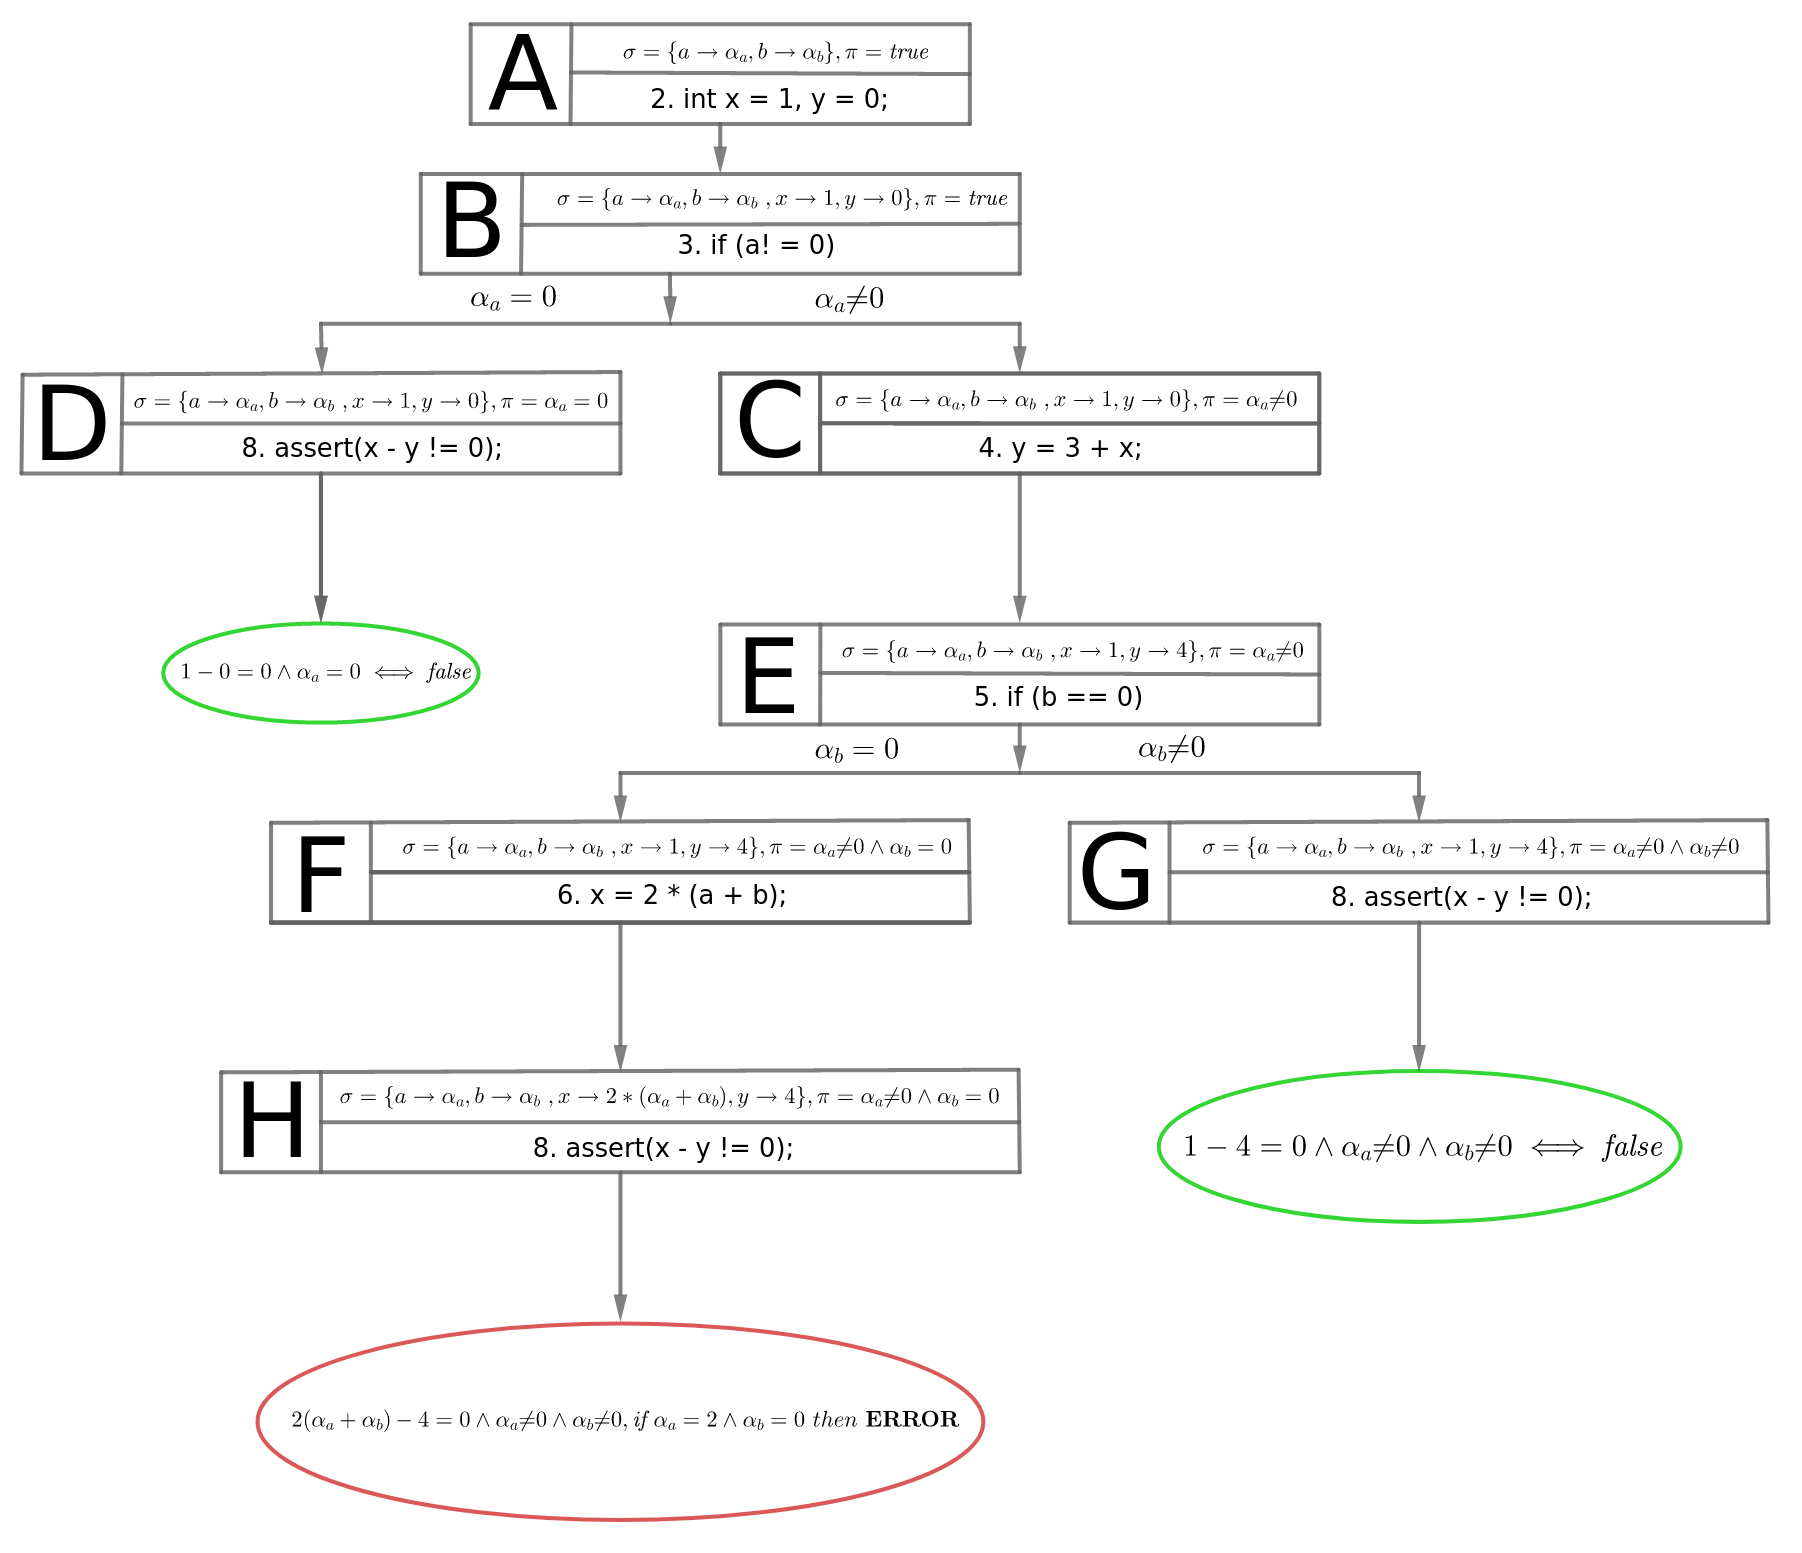
\includegraphics[width=1.0\linewidth]{osnovni_primer.png}
    \caption{Stablo stanja simboličkog izvršavanja koje odgovara primeru \ref{lst:osnovni_primer}. Crvenom elipsom je predstavljeno završno stanje kod koga može doći do greške, dok su zelenim elipsama označena završna stanja kod kojih nema grešaka.}
    \label{fig:osnovni_primer}
\end{figure}

Graf simboličkog izvršavanja može biti predstavljen stablom, što se je prikazano na slici \ref{fig:osnovni_primer}. Incijalno u korenu stabla (stanje $A$) imamo formulu $\pi$ koja ima vrednost \textbf{tačno} (eng. \textit{true}), i promenljivima $a$ i $b$ su dodeljene simboličke vrednosti $\alpha_a$ i $\alpha_b$. Stanje $B$ odgovara prvoj naredbi unutar funkcije $foo$ u kojoj se promenljivima $x$ i $y$ dodeljuju vrednosti 1 i 0 redom, čime one postaju konkretne promenljive. U stanju $B$ se memorijski prostor $\sigma$ ažurira tako što se menjaju vrednosti promenljivih $x$ i $y$. Sledeća naredba je naredba grananja pa se stanje $B$ deli na dva stanja, $C$ i $D$. Stanja $C$ i $D$ odgovaraju uslovima $\alpha_a \neq 0$ i $\alpha_a = 0$ redom, što se može i videti na osnovu ažuriranja formule $\pi$ u odgovarajućim stanjima. Daljom analizom se može zaključiti da su stanja $D$, $G$ i $H$ završna stanja, tj. stanja u kojima se izvršava poslednja naredba funkcije $foo$. Jedina formula koja može dovesti do greške je ona u stanju $H$. Bilo koje ulazne vrednosti za simboličke promenljive $a$ i $b$ za koje važi
\vskip 0.2in
\centerline{$2(\alpha_a + \alpha_b) - 4 = 0 \land \alpha_a \neq 0 \land \alpha_b = 0$}
\vskip 0.2in
\noindent će dovesti do narušavanja uslova naredbe $assert$. Vrednosti koje bi dovele do greške se mogu odrediti pozivanjem $SMT$ rešavača, u datom primeru to su vrednosti \texttt{a = 2} i \texttt{b = 0}.

\section{Metode simboličkog izvršavanja}
Teorijska ideja simboličkog izvršavanja je da se istraže sve moguće putanje u okviru nekog koda (softvera) i da se odrede odgovarajuće kombinacije ulaznih podataka koje bi dovele do grešaka. U praksi to nije moguće zbog eksplozije stanja i ograničene memorije računara, pa samim tim alati za simboličko izvršavanje ne pretražuju sve moguće putanje. 

Jedan od dodatnih problema je i što u realnom softveru postoji k\^od iz eksternih biblioteka kojima sam alat nema pristup, pa samim tim ne može da generiše sve putanje kroz taj deo koda. Sporedni efekti prilikom izvršavanja koda (kako programski koji se tiču simboličkih promenljivih tako i neki drugi koji se tiču arhitekture računara) mogu predstavljati problem pri rekonstrukciji kompletnog steka softvera koji se analizira. Osnovna ideja za rešavanje ovih problema je kombinovanje konkretnog i simboličkog izvršavanja, takozvano \textit{konkoličko izvršavanje} (eng. \textit{concolic}), što je kovanica reči \textit{concrete} i \textit{symbolic}.

\subsection{Dinamičko simboličko izvršavanje}
Jedna od popularnih metoda konkoličnog simboličkog izvršavanje je dinamičko simboličko izvršavanje (eng. \textit{Dynamic Symbolic Execution} ili $DSE$). Ideja ovog pristupa je da simboličko izvršavanje bude vođeno konkretnim izvršavanjem. 

Pored simboličkog memorijskog prostora i formula koje predstavljaju ograničenja na različitim putanjama, alat za simboličko izvršavanje čuva i konkretan memorijski prostor $\sigma_c$. Na početku izvršavanja je potrebno odrediti konkretne vrednosti za ulazne podatke, a zatim se sam k\^od izvršava i konkretno i simbolički, paralelno ažurirajući oba memorijska prostora i odgovarajuća ograničenja koja odgovaraju putanjama. Kada se naiđe na naredbu grananja, na osnovu konkretnih vrednosti promenljivih se određuje kojom granom se nastavlja izvršavanje. Granu koja se bira konkretnim izvršavanjem bira i simboličko izvršavanje i na odgovarajući način se ažurira formula $\pi$ koja odgovara putanji. Dakle, simboličko izvršavanje prati konkretno izvršavanje. 

Ovakav način izvršavanja omogućava da SMT rešavač ne mora da se poziva nakon svakog grananja kako bi se proverilo da li je formula koja se dobija dodavanjem izraza koji odgovara izabranoj putanji nezadovoljiva, jer se to rešava konkretnim izvršavanjem, s obzirom da su konkretne vrednosti promenljivih poznate. Kako bi se istraživale različite putanje, moguće je negirati uslov nekog od grananja i pozvati SMT rešavač kako bi odredio koje su vrednosti ulaznih podataka koje bi dovele do kretanja baš tom putanjom, odnosno koje početne vrednosti ulaznih podataka odgovaraju negiranom uslovu u naredbi grananja. 

Razmotrimo primer koji je dat listingom \ref{fig:osnovni_primer}. Neka su ulazne vrednosti \texttt{a = 1} i \texttt{b = 1}. Izvršavanje bi krenulo od stanja $A$, 
zatim se prelazi u stanje $B$ gde postoji grananje.
Kako je uslov \texttt{a != 0} ispunjen, izvršavanje bi nastavilo stanjem $C$, nakon čega se nastavlja stanjem $E$ u kome opet imamo grananje. S obzirom da uslov $b == 0$ nije ispunjen (jer imamo konkretnu vrednost promenljive $b$ koja je $1$), izvršavanje ulazi u završno stanje $G$. 
Konkretan memorijski prostor se kroz ovo izvršavanje menja na sledeći način:
\begin{itemize}
    \item $\sigma_c = {a \rightarrow 1, b \rightarrow 1}$ u stanju $A$,
    
    \item $\sigma_c = {a \rightarrow 1, b \rightarrow 1, x \rightarrow 1, y \rightarrow 4}$ u stanjima $B$ i $C$ i
    
    \item $\sigma_c = {a \rightarrow 1, b \rightarrow 1, x \rightarrow 1, y \rightarrow 0}$ u stanjima $E$ i $G$.
\end{itemize}
U stanju $G$ može da se ustanovi da je sve u redu, tj. nema narušavanja ograničenja koje je zadato naredbom $assert$, pa se nova putanja može generisati negacijom nekog od uslova koji su bili ispunjeni u naredbama grananja. Recimo da se negira uslov $\alpha_b \neq 0$. SMT rešavač će generisati nove ulazne podatke koji  zadovoljavaju ovaj uslov, recimo \texttt{a = 1\texttt}, \texttt{b = 0} i na taj način je otkrivena nova putanja. U ovom slučaju bi izvršavanje išlo kroz stanja $A \rightarrow B \rightarrow C \rightarrow E \rightarrow F$.

Iako dinamičko simboličko izvršavanje počinje dodelom konkretnih vrednosti promenljivima, nove putanje se generišu negiranjem određenih uslova. Potrebno je odabrati uslov koje naredbe grananja će biti negiran. Broj naredbi grananja (samim tim i broj različitih putanja) u nekom kodu može biti jako veliki, s toga je neophodno na neki način vršiti odabir uslova koji će biti negirani jer je nemoguće u razumnom vremenu proći kroz sve putanje. Načini na koje različiti alati koji vrše dinamičko simboličko izvršavanje biraju koji će uslov biti negiran će biti diskutovan dalje u tekstu. 

U nekim situacijama alat za simboličko izvršavanje koji radi na principu dinamičkog simboličkog izvršavanja ne može da isprati ceo k\^od simbolički. Razlog za to može da bude poziv funkcije koja je deo neke eksterne biblioteke čiji izvorni k\^od nije dostupan. 
Razmotrimo primer čiji je k\^od prikazan kroz listing \ref{lst:eksterna_1}

\bigbreak
    \begin{lstlisting}[caption={Primer gde rezultat izvršavanja eksterne funkcije nije važan},captionpos=b,label={lst:eksterna_1}]
        void foo(int a, int b)
        {
          int x = bar(a);
          
          if (b > 5)
            ERROR;
        }
    \end{lstlisting}
\bigbreak

Alat u ovom slučaju promenljivima $a$ i $b$ dodeljuje slučajne vrednosti na početku izvršavanja funkcije $foo$. Pretpostavimo da važi \texttt{a = 1} i \texttt{b = 0}. Sva grananja i sve naredbe koje se izvršavaju u okviru funkcije $bar$ su potpuno nepoznate alatu. Kako bi se otkrila neka nova, potencijalno zanimljiva putanja, potrebno je negirati neki od uslova u grananjima kroz koja se prolazi tokom izvršavanja koda. Jedino grananje koje je poznato je \texttt{if (b > 5)} (izvorni k\^od funckije $bar$ nije dostupan), tako da je moguće negirati uslov baš tog grananja. Na taj način se pomoću SMT rešavača dobijaju novi ulazni podaci za koje mora da važi \texttt{b > 5}, recimo \texttt{a = 1} i \texttt{b = 7}. Na ovaj način se otkriva nova putanja, i otkriva se da može doći do greške u izvršavanju navedene funkcije.

\bigbreak
    \begin{lstlisting}[caption={Primer gde je rezultat izvršavanja eksterne funkcije važan},captionpos=b,label={lst:eksterna_2}]
        void foo(int a)
        {
          int x = bar(a);
          
          if (x > 0)
            ERROR;
        }
    \end{lstlisting}
\bigbreak

Posmatrajmo primer prikazan kroz listing \ref{lst:eksterna_2}. Pretpostavimo da izvorni k\^od funkcije $bar$ nije poznat ni u ovom slučaju. Ono što se primećuje je da uslov grananja koje je poznato direktno zavisi od rezultata njenog izvršavanja. Recimo da je alat za simboličko izvršavanje generisao ulazne podatke (vrednost za simboličku promenljivu $a$) tako da uslov poznate naredbe grananja nije poznat. SMT rešavač pokušava da negira uslov i generiše nove ulazne podatke koji treba da omoguće otkrivanje nove putanje. Međutim, kako izvorni k\^od funkcije $bar$ nije poznat a uslov grananja direktno zavisi od rezultata njenog izvršavanja nije moguće garantovati da će generisanjem novih ulaznih vrednosti biti otkrivena putanja koja može dovesti do greške. U nekim situacijama je alatu nemoguće da otkrije da ne postoje ulazni podaci koji mogu otkriti novu putanju, tj. da postoji nedostižan kod. Taj slučaj je ilustrovan primerom čiji je k\^od dat listingom \ref{lst:eksterna_3}.

    \begin{lstlisting} [caption={Primer u kome može doći do divergencije putanje},captionpos=b,label={lst:eksterna_3}]
        void foo(int a)
        {
          double x = pow(a, 2);
          
          if (x < 0)
            ERROR;
        }
    \end{lstlisting}
\bigbreak

U ovom primeru imamo slučaj gde funkcija $foo$ poziva funkciju $pow$ koja vraća kvadrat svog prvog argumenta. Neka je alat generisao $a = 5$ kao ulazni podatak. Kako uslov u naredbi grananja nije ispunjen, rešavač će otkriti da je potrebno negirati uslov $a \geq 0$. Novi ulazni podatak bi mogao da bude $a = -5$. Međutim, ni na ovaj način se neće desiti da je uslov u naredbi grananja ispunjen. Alat nema mogućnost da otkrije da je nemoguće da dođe do greške, tj. da je naredba u kojoj dolazi do greške nedostižna. 

Na osnovu prethodnih primera možemo videti da postoje problemi u dinamičkom simboličkom izvršavanju. Neotkrivanje nekih interesantnih putanja, nemogućnost otkrivanja nedostižnog koda. Pozivi eksternih funkcija, kastovanje i simboličkli pokazivači su neki od najvažnijih aspekata o kojima se mora voditi računa prilikom dinamičkog simboličkog izvršavanja kako ne bi došlo do divergencije putanja.\footnote[2]{Divergencija putanja je pojava u dinamičkom simboličkom izvršavanju gde izvršavanje vodi nekom neočekivanom putanjom. Recimo u primeru \ref{lst:eksterna_3} bi bilo očekivano da negacijom uslova grananja bude otkrivena nova putanja, međutim to se nikada neće desiti jer je kvadrat bilo kog broja uvek pozitivan broj.}

\subsection{Selektivno simboličko izvršavanje}
Postoji i drugačiji pristup konkoličkom simboličkom izvršavanju koji vrši alat za selektivno simboličko izvršavanje (eng. \textit{Selective Symbolic Execution} ili $S^2E$). Kod ovog alata simboličko i konkretno izvršavanje se kombinuju na drugačiji način u odnosu na dinamičko simboličko izvršavanje. Neka postoje dve funkcije $A$ i $B$ pri čemu funkcija $A$ poziva funkciju $B$.
Postoje dva osnovna pristupa:
\begin{enumerate}
    \item \textbf{od konkretnog ka simboličkom i nazad} - funkcija $A$ se izvršava konkretno. Kada se dođe do narebe u kojoj se poziva funkcija $B$, argumenti funkcije se prave simboličkim kako bi se cela funkcija simbolički izvršila i otkrile eventualne greške u istoj. Funkcija $B$ se takođe izvršava i konkretno, a zatim se rezultat konkretnog izvršavanja vraća funkciji $A$ kako bi ona nastavila da se izvršava konkretno.
    
    \item \textbf{od simboličkog ka konkretnom i nazad} - funkcija $A$ se izvršava simbolički. Kada se dođe do narebe u kojoj se poziva funkcija $B$, argumenti funkcije se konkretizuju i funkcija se u potpunosti izvršava konkretno. Nakon izvršavanja funkcije $B$, izvršavanje se vraća na funkciju $A$ koja se nastavlja simbolički.
\end{enumerate}

Ovakav pristup utiče i na saglasnost i na kompletnost rezultata.

\begin{description}
    \item \textbf{kompletnost} - potrebno je na neki način izbeći lažno pozitivne rezultate. Kada se funkcija $B$ izvršava simbolički potrebno je voditi računa kroz koje je grane moguće proći zavisno od konkretizacije argumenata, jer izvršavanje funkcije $B$ direktno zavisi od vrednosti promenljivih u funkciji $A$. Kod selektivnog simboličkog izvršavanja se pri kreiranju formule određene putanje u simboličkom izvršavanju ($\pi$) vodi računa o načinu na koji su argumenti konkretizovani, koje vrednosti mogu da uzmu, koji su to sporedni efekti koji mogu da se dese u funkciji $B$ i koja će biti povratna vrednost funkcije za konkretne vrednosti argumenata.
    
    \item \textbf{saglasnost} - takođe može da dođe do lažno negativnih rezultata što je potrebno izbeći. S obzirom da se argumenti funkcije $B$ konkretizuju nakon povratka u funkciju $A$ je moguće da se kroz neka grananja ne prolazi. Kako bi se ovaj problem rešio, funkcija $B$ se konkretno izvršava veći broj puta, pri čemu se za svako od izvršavanja vodi računa kojom putanjom se prošlo kroz funkciju $B$, i nove konkretne ulazne vrednosti parametara se biraju tako da se kroz $B$ u svakom sledećem izvršavanju ide kroz neke nove putanje.
\end{description} 
\bigskip
\subsection{Simboličko izvršavanje unazad} 
Još jedan vid simboličkog izvršavanja je simboličko izvršavanje unazad (eng. \textit{Symbolic Backward Execution} ili \textit{SBE}). Osnovna ideja ovog pristupa je da se krene od neke naredbe u kodu i da se izvršavanje kreće ka ulazu, tj. početku rada programa. Ova tehnika se obično koristi kada je potrebno odrediti pod kojim uslovima se može doći do neke konkretne naredbe u kodu, i kojom se putanjom do nje stiže. Osnovna mana ovog pristupa je što je neophodno da postoji graf (stablo) izršavanja samog programa, a konstrukcija tog grafa je često izuzetno skupa i komplikovana operacija.

\section{Algoritmi simboličkog izvršavanja}

Postoji veliki broj algoritama i heuristika koje koriste alati za simboličko izvršavanje. U ovom delu će biti dat njihov kratak prikaz.

\bigbreak

\subsection{Pretraga grafa u dubinu} \label{DFS}
Jedan od osnovnih i najpoznatijih algoritama koji se koriste u simboličkom izvršavanju je pretraga grafa u dubinu (eng. \textit{Depth-First Search} ili $DFS$). Kako simboličko izvršavanje koda možemo predstaviti kao stablo stanja kroz koja se prolazi, a s obzirom da je stablo zapravo aciklički graf, možemo koristiti algoritme za pretragu grafova kako bismo birali sledeće stanje koje će biti izvršavano. Algoritam DFS bira putanju kojom kreće inicijalno, prilikom prvog grananja, zatim tu putanju istražuje do kraja. Ide maksimalno u dubinu sve dok se ne dođe do kraja putanje ili dok ne bude ispunjen neki drugi uslov zaustavljanja (dubina rekurzije, broj naredbi koje su izvršene na putanji, vreme koje je provedeno istražujući određenu putanju itd). Nakon toga algoritam vrši odsecanje te putanje, vraća se unazad do nekog prethodnog grananja i nastavlja drugim putem. Zatim se ta nova putanja istražuje maksimalno (do kraja, ili nekog drugog uslova izlaska). 

Algoritam pretrage grafa u dubinu se obično koristi kada je memorija kojom se raspolaže ograničena (nedovoljno velika za čuvanje velikog broja stanja). Najveća mana ovog pristupa je što jako dugo radi kada u kodu postoji rekurzivna funkcija koja se izvršava ili ukoliko postoje petlje čije ograničenje nisu konkretne vrednosti već simboličke promenljive. 

\bigbreak

\subsection{Pretraga grafa u širinu} \label{BFS}
U simboličkom izvršavanju se za pretragu stabla stanja često koristi i drugi grafovski algoritam, pretraga grafa u širinu (eng. \textit{Breadth-First Search} ili $BFS$). Pretraga u širinu ima prednosti u odnosu na pretragu u dubinu jer paralelno izučava veliki broj putanja. Na ovaj način se mogu otkriti neka zanimljiva opažanja ranije u odnosu na pretragu u dubinu i češće se koristi ukoliko je vreme ograničeno (previše kratko da bi se čekalo da DFS pretraga istraži jednu po jednu putanju do kraja). 

Mana ovog algoritma je to što čuva ogroman broj stanja i puni memoriju koja je dodeljena alatu za simboličko izvršavanje. Pošto se veliki broj putanja paralelno izučava potrebno je za sve njih čuvati stanja, formule logike prvog reda čija se zadovoljivost proverava SMT rešavačem (ograničenja koja važe za svaku od putanja), održavati simbolički memorijski prostor i slično. Iz navedenih razloga je potrošnja memorije znatno veća u odnosu na algoritam pretrage u dubinu. Još jedna mana ovog pristupa je što nije realno očekivati da sve putanje mogu biti izučene do kraja. 

Vreme je često ograničavajući faktor kada govorimo o analizi realnog softvera gde postoji jako veliki broj linija koda pa u tim situacijama algoritam pretrage u širinu ne uspeva da izuči sve putanje do kraja. Međutim, činjenica je da se paralelnim izučavanjem većeg broja putanja lakše i brže dolazi do interesantnih zapažanja u odnosu na pretragu u dubinu.

\bigbreak

\subsection{Slučajan odabir narednog stanja} 
Slučajan odabir narednog stanja je strategija kod koje se naredno stanje koje će biti obrađeno bira na potpuno slučajan način. Od svih trenutno dostupnih stanja u stablu pretarge na slučajan način se bira jedno od njih. Ova ideja je sama po sebi jako loša jer nema konkretne strategije po kojoj bira sledeće stanje, međutim često se dodatno obogaćuje različitim heuristikama. 

Neke poznate heuristike su:

\begin{description}
    \item \textbf{Izvršavanje vođeno pokrivenošću koda} - osnovna ideja ove heuristike je da se za svaku putanju određuje njena važnost na osnovu toga koliko naredbi je u određenoj putanji izvršeno od otkrivanja poslednje nove naredbe, koliko je udaljena naredna neposećena naredba i slično.
    
    \item \textbf{Izvršavanje vođeno podputanjama} - ideja je birati ono stanje koje vodi podputanjom koja je bila izvršena manji broj puta do tog trenutka. Podputanja se definiše kao $n$ uzasptonih naredbi u okviru jedne putanje. Kod ove heuristike ključnu ulogu igra odabir vrednosti $n$. Do sada nije pronađena optimalna vrednost parametra $n$ koja je univerzalna.
    
    \item \textbf{Izvršavanje stanja najbližeg naredbi} - ova heuristika se obično koristi kada je potrebno doći do određene naredbe u samom kodu. Uvek se bira ono stanje koje je najbliže traženoj naredbi. Malo podseća na pretragu vođenu pokrivenošću koda, međutim razlika je u tome da u ovoj strategiji težimo jednoj konkretnoj naredbi, a ne pokrivenosti celokupnog koda.
    
    \item \textbf{Iscrpljivanje petji} - osnovna ideja ove heuristike je da se biraju putanje koje sadrže petlje. Opravdanje se krije u opažanju da u praksi veliki broj grešaka u radu sa petljama vodi ka prekoračenju bafera\footnote[3]{Prekoračenje bafera je pojva gde prilikom upisivanja podataka u bafer dolazi do pisanja van njegovih granica. Odnosno, podaci se smeštaju na susedne lokacije, u memoriju gde ne bi trebalo da se nalaze.} i drugim memorijskim problemima.
    
    \item \textbf{Prvo putanje sa greškama} - kod ove heuristike se prvo izučavaju one putanje kod kojih su u nekim ranijim delovima pronađene sitne greške (eng. \textit{bugs}). Intuicija iza ovog pristupa je da ako je putanja u ranijem delu imala neku grešku nije dovoljno dobro istestirana.
\end{description}

\subsection{Generacijska pretraga} 
Ova tehnika uglavnom predstavlja kombinaciju pretrage u dubinu i pretrage vođene pokrivenošću koda. Osnovna ideja je da se pretraga vrši po generacijama. Kreće se od nulte generacije u kojoj se slučajno odabrana putanja izvršava do kraja pomoću algoritma pretrage grafa stanja u dubinu. U prvoj generaciji se iz putanje nulte generacije istražuju nove putanje i to tako što se odredi jedan od uslova grananja u putanji nulte generacije i njegovim negiranjem se dobija sledeća putanja. U $n$-toj generaciji se iz svih putanja prethodne generacije bira uslov koji se negira i pomoću koga se kreće u istraživanje nove putanje. Biranje putanje kojom će se krenuti se vrši heuristikom vođenom pokrivenošću koda.
\bigskip

\subsection{Hibridne strategije} 
Hibridne strategije se svode na kombinaciju većeg broja algoritama koji se na određene načine smenjuju prilikom pretrage. Zavisno od specifičnih potreba (otkrivanje putanje do određene naredbe, otkrivanje što većeg broja putanja, pokrivenost koda itd.) koriste se kombinacije različitih algoritama koji se pri izvršavanju smenjuju i kombinuju na različite načine.

\section{Karakterisitike alata za simboličko izvršavanje} \label{osobine_alata}

Postoji veliki broj različitih alata za simboličko izvršavanje. Većina ovih alata počiva na istim principima:

\begin{description}
    \item \textbf{Napredak} - izvršavanje bi trebalo da može da traje neko određeno vreme bez potrošnje svih resursa koji su mu dodeljeni. Tu se pre svega misli na memoriju koja često može biti resurs koji biva brzo iskorišćen u potpunosti zbog velikog broja raličitih putanja i stanja.
    
    \item \textbf{Ponovljen posao} - ne bi trebalo da se neki posao ponavlja. Odnosno, nije dobro da se izvršavanje pokreće od samog početka da bi se otkrile neke nove putanje ako već postoji zajednički prefiks te putanje sa nekim postojećim. Rezultati prethodnih izračunavanja i saznanja iz prethodnih putanja bi trebalo da se koriste u što većoj meri kako bi se uštedelo vreme, i smanjilo ponavljanje posla. Tu se pre svega misli na skupe pozive SMT rešavaču za formule za koje je zadovoljivost proverena ranije. Takve pozive treba izbegavati.
    
\end{description}
\bigskip
Na osnovu toga da li pokušavaju da obrade veći broj putanja odjednom ili jednu po jednu alati za simboličko izvršavanje se mogu podeliti u dve grupe:
\begin{description}
    \item \textbf{\textit{online} alati} - alati koji pokušavaju da izvršavaju i izučavaju veći broj putanja odjednom. Kada god se naiđe na grananje vrši se kloniranje trenutnog stanja. Dobra strana ovih alata je što nema ponavljanja posla jer se jednom izvršena naredba nikada ne izvršava ponovo. Loša strana je to što veoma brzo pune memoriju koja im je dodeljena, jer moraju da održavaju veliki broj putanja i stanja. Na primer ako imamo uslov grananja $x > 3$, putanja se deli na dve disjunktne putanje. U jednoj će važiti $\pi \land x > 3$ a u drugoj negacija tog uslova, odnosno $\pi \land x \leq 3$. Na ovaj način se prolazi kroz obe putanje. Primeri ovakvih alata su KLEE \cite{klee}, AEG \cite{aeg}, S$^2$E \cite{s2e}.
    
    \item \textbf{\textit{offline} alati} - za razliku od \textit{online} alata, \textit{offline} alati izvršavaju jednu po jednu putanju. Primer ovakvog alata je SAGE \cite{sage}. Ideja je izvršiti celu jednu putanju do samog kraja, a zatim preći na neku drugu. Dobra strana ovog pristupa je jako malo korišćenje memorije jer se čuvaju stanja vezana za samo jednu putanju, ali je problem što obično ima mnogo ponavljanja posla. Pretraga nove putanje uglavnom kreće od samog početka. Opšti princip rada \textit{offline} alata je da kreću sa konkretnim izvršavanjem, što znači da je potrebno generisati ulazne podatke. Pamti se put kojim se prošlo pri konkretnom izvršavanju, a zatim se isti put prolazi simbolički. 
    
    \item \textbf{\textit{hibridni} alati} - hibridni alati kao što je Mayhem \cite{mayhem} pokušavaju da pronađu balans između prevelikog utroška memorije i vremena koje je potrebno za izvršavanje. Na početku počinju kao \textit{online} rešavači, a kada se memorija popuni do određene količine prelaze u \textit{offline} izvršavanje.
\end{description}

\section{Pregled najpoznatijih alata za simboličko izvršavanje} \label{alati_za_simbolicko}

U daljem tekstu će biti ukratko opisani alati koji simboličkim izvršavanjem vrše verifikaciju softvera.

\paragraph{DART}\cite{dart} (eng. \textit{Directed Automated Random Testing}) je alat koji vrši dinamičko konkoličko simboličko izvršavanje. Za odabir uslova grananja koji će biti negiran kako bi se otkrila nova putanja se koristi algoritam pretrage u dubinu (DFS). DART je alat koji počiva na tri osnovna principa:
\begin{enumerate}
    \item\textit{Automatski} izdvaja interfejs programa statičkom analizom izvornog koda.
    
    \item\textit{Slučajno} (eng. \textit{Random}) generiše testove za izdvojeni interfejs programa kako bi se simuliralo što opštije okruženje rada programa.
    
    \item Analizom ponašanja programa i automatskim generisanjem novih test primera, izvršavanje se \textit{usemrava} (eng. \textit{Direct}) ka drugim mogućim putanjama.
\end{enumerate}

\noindent DART se uglavnom koristi za testiranje programa napisanih u programskom jeziku \textit{C}.

\paragraph{SAGE}\cite{sage} je alat koji vrši dinamičko simboličko izvršavanje. Za razliku od DART$-$a, SAGE koristi generacijsku pretragu. Osnovna ideja ovog alata je da sistematski, ali ipak delimično istraži prostor mogućih stanja softvera pri čemu se izbegava ponavljanje posla, a ujedno maksimizuje broj generisanih različitih testova. Pošto se izučava samo deo prostora stanja, ključan je izbor ulaznih vrednosti simboličkih promenljivih. Važnost inicijalnih vrednosti podseća na važnost istih kod tradicionalnog rasplinutog testiranja metodom crne kutije (eng. \textit{black-box fuzzy testing}), pa se stoga alati poput SAGE$-$a često nazivaju rasplinutim testerima metodom bele kutije (eng. \textit{white-box fuzzy testers}). SAGE je primer \textit{offline} alata. 

\paragraph{S$^2$E}\cite{s2e} je alat koji vrši selektivno simboličko izvršavanje. Jedan je od glavnih predstavnika \textit{online} alata. Pored ranije navedenih osobina treba napomenuti da se za izbor narednog stanja koje se izvršava, samim tim i izbor putanje koja se izučava, vrši heuristikom vođenom pokrivenošću koda. 

\paragraph{Mayhem}\cite{mayhem} je primer \textit{hibridnog} alata za simboličko izvršavanje. Ovaj alat kombinuje tehnike \textit{online} i \textit{offline} alata i to tako što koristi prednosti svake od tehnika. Ova jalat radi direktno sa izvršnim kodom. Kako bi ovo bilo moguće postoje dve važne stavke o kojima Mayhem mora da vodi računa:
\begin{itemize}
    \item Održavanje putanja koje se izučavaju bez potpune potrošnje dostupne memorije.
    
    \item Oprez pri radu sa simboličkom memorijom, odnosno sa simboličkim adresama kako ne bi dolazilo do prekoračenja bafera i sličnih problema.
\end{itemize} 
\medskip
Pored koncepta hibridnog alata, Mayhem još uvodi i memoriju zasnovanu na indeksima, tehniku koja ovom alatu omogućava da efikasno radi sa simboličkom memorijom na binarnom nivou (rad sa izvršnim fajlovima).

\paragraph{AEG}\cite{aeg}, odnosno \textbf{Automatic Exploit Generation} je alat koji je napravljen kao nadgradnja drugog alata za simboličko izvršavanje, \textit{KLEE-a}\cite{klee}. Osnovna ideja ovog alata je da se ne istražuju sve moguće putanje u programu, već da fokus bude na onim putanjama za koje se veruje da imaju veću verovatnoću izvršavanja zavisno od vrednosti ulaznih podataka. Osnovna tehnika kojom se služi ovaj alat je preduslovno simboličko izvršavanje (eng. \textit{preconditioned symbolic execution}). Jedan zasad poznati problem ovog alata je skalabilnost na velikim programima, ali se na tome aktivno radi.

\paragraph{KLEE}\cite{klee} je jedan od najkorišćenijih alata za simboličko izvršavanje. Kako je ovaj rad zasnovan upravo na alatu KLEE, on će biti detaljnije opisan u delu \ref{KLEE}.

\chapter{Alat za simboličko izvršavanje KLEE} \label{KLEE}
\paragraph{KLEE}\cite{klee} je alat otvorenog koda koji je nastao na Univerzitetu Ilinois. U pitanju je potpuno simbolički alat što znači da su sve promenljive simboličke i nema konkoličkog simboličkog izvršavanja. Ideja alata je da pokuša kompletne programe da izvršava simbolički uz dodatak konkretnih vrednosti koje se u kodu javljaju kao konstante. Dakle, KLEE ne generiše slučajan ulaz i na taj način prati kojim se putem prolazi zavisno od vrednosti, već pokušava da ide različitim putevima odjednom menjajući uslove koji važe. U pitanju je \textit{online} alat, čija je odlika da sve putanje obilazi paralelno, tj. ne izučava jednu putanju do kraja. Stanja koja su vezana za svaku od aktivnih putanja se čuvaju sve vreme bez obzira na algoritam koji se koristi.

\section{Memorijski model} \label{memorija}
KLEE čuva vrednosti različitih promenljivih u skladištima. Postoje dva skladišta u okviru alata. 
\begin{description}
    \item \textbf{konkretno} - skladište u okviru kog se čuvaju vrednosti konkretnih promenljivih. To su konstante ili promenljive kojima je dodeljena vrednost u kodu. Na primer, naredba \texttt{int x=5;} definiše jednu konkretnu promenljivu. Ukoliko se desi da se vrši dodela vrednosti konkretnoj promenljivoj kao rezultat izračunavanja u kome je učestvovala simbolička promenljiva, onda i konkretna promenljiva postaje simbolička. S druge strane, ukoliko se vrši neko izračunavanje nad simboličkom i konkretnom promenljivom, a rezultat se dodeljuje simboličkoj promenljivoj, to ne utiče na konkretnu promenljivu, i ona ostaje kakva je i bila pre ovog izračunavanja.
    
    \item \textbf{simboličko} - skladište gde se čuvaju simboličke promenljive. Kako one nemaju konkretne vrednosti sve do trenutka kada se dođe u završno stanje, veći deo vremena se čuva samo njihova adresa. Kada se dođe u završno stanje, potrebno je generisati konkretne vrednosti simboličkih promenljivih na osnovu uslova koji važe u tom stanju. U tom trenutku one dobijaju konkretne vrednosti, i generiše se test primer koji govori o tome koje su vrednosti promenljivih kada se program izvrši kretanjem kroz određenu putanju. Te vrednosti ne moraju biti jednistvene, npr ako u stanju važi uslov $x > 5$ promenljiva $x$ može uzeti bilo koju vrednost koja je veća od $5$. Ukoliko u nekom stanju dolazi do greške pod uslovom $x = 7$ onda će vrednost promenljive $x$ koja se generiše u tom stanju biti baš $7$.
\end{description}
\bigskip
Količina radne memorije koja se dodeljuje samom alatu je ograničena i zadaje se kao jedan od parametara prilikom pokretanja samog KLEE-a. Zbog osobine alata da čuva sva stanja koja su vezana za sve putanje koje se izučavaju vrlo često dolazi do situacije gde se memorija popuni. Kada se ovo desi na neki način mora da dođe do ,,pražnjenja''. To se radi tako što se odbacuju neka stanja. Broj stanja koja se izbacuju se određuje slučajnom metodom. Generiše se pseudo-slučajan broj i on predstavlja broj stanja koja se izbacuju. 
Neophodno je definisati na koji način se biraju stanja koja bivaju izbačena. Ovaj postupak je takođe slučajan uz još jedan dodatan uslov, a to je da se ne izbacuju stanja koja su otkrila novu naredbu. Generiše se pseudo-slučajan broj koji govori o indeksu stanja u nizu koje treba da bude izbačeno i ako u njemu nije otkrivena nova naredba ono može biti izbačeno. U suprotnom se generiše nov indeks i bira se drugo stanje za izbacivanje iz skupa aktivnih stanja.

\section{Kontrola toka programa}
Rad sa funkcijama u alatu KLEE liči na standardni rad sa funkcijama u nekom programskom jeziku. Ukoliko je potrebno simbolički izvršiti funkciju $f$, koja se poziva iz funkcije $g$ sa parametrom $a$ bez povratne vrednosti (\texttt{void f(int a)}), izvršavanje se vrši na sledeći način. U okviru alata postoji ,,stek'' na kome se čuvaju lokalne promenljive i parametri funkcije $f$. Takođe se pamti koja je funkcija pozivalac kao i koju naredbu funkcije $g$ treba izvršiti nakon što $f$ bude izvršena. Sve promenljive se i dalje čuvaju u ranije opisanim skladištima. Nakon što se završi izvršavanje funkcije, memorija na kojoj su se nalazile lokalne promenljive postaje ,,slobodna'', odnosno tu je moguće smeštati nove promenljive neke nove funkcije. 

Ovo važi za funkcije za koje je izvorni k\^od poznat i napisan u programskim jezicima C i C++. Može se desiti je da izvorni k\^od neke funkcije nije poznat, ili da je napisan u drugom programskom jeziku. U ovom slučaju KLEE nije u mogućnosti da prati izvršavanje funkcije simbolički. Tada se argumenti konkretizuju na osnovu uslova koji važe na putanji gde se nalazi poziv funkcije i funkcija se poziva i čuva se povratna vrednost ukoliko postoji. Ukoliko funkcija koja je pozvana nema povratnu vrednost, ona se izvršava bez simboličkog praćenja i izvršavanje se nastavlja simbolički u okviru funkcije pozivaoca. 

\indent Kada je reč o petljama, KLEE ima prilično specifičan način rada. Naime, kako je alat potpuno simbolički, sve petlje se izvršavaju do kraja kroz sve potencijalne iteracije. Ako važi da je uslov izlaska iz petlje \texttt{i < n} gde je $n$ simbolička promenljiva, KLEE će pokušavati da prođe sve moguće iteracije. Ukoliko bi se znalo da je vrednost promenljive $n$ na primer $1000$ onda bi se petlja vrtela simbolički do vrednosti 1000. Međutim, kada je granica broja iteracija petlje simbolička promenljiva, KLEE nema mogućnost da izvrti određen broj iteracija i vidi ponašanje programa, već se ide do maksimalne vrednosti koju može da čuva promenljiva tipa koji odgovara tipu promenljive $n$. Iz ovog razloga KLEE ima veliki problem sa petljama bez obzira na to koji se algoritam koristi. Često u okviru petlji postoje grananja što dovodi do toga da se kreira veliki broj novih stanja u okviru njih. Na ovaj način se i memorija brže puni što dovodi do potrebe za ranije opisanim odbacivanjem nekih stanja. 

Kada se govori o rekurzivnim funkcijama situacija je veoma slična. Rekurzija se izvršava do uslova izlaska. Ukoliko uslov izlaska iz rekurzije zavisi od simboličke promenljive, javlja se isti problem kao i pri radu sa petljama.

\section{Rad sa pokazivačima i nizovima}
Praćenje vrednosti pokazivača liči na rad sa pokazivačima u programskom jeziku C. Postoji poseban deo memorije koji se zove \textit{Known Symbolics} gde se smeštaju promenljive poslate funkciji preko pokazivača. Kada je promenljiva prosleđena preko pokazivača funkciji, nju je moguće menjati u okviru te funkcije. Ako je u pitanju simbolička promenljiva potrebno je znati koja simbolička promenljiva se ,,menja'', tj. koji dodatni uslovi za tu promenljivu treba da važe. Zato postoji pomenuti deo simboličkog skladišta koji čuva sve simboličke promenljive koje su uvedene do tad. Objekat pokazivačke promenljive koja se kreira prilikom poziva funkcije kao jedno od polja čuva i adresu promenljive na koju ,,pokazuje''. Na taj način je moguće u okviru dela \textit{Known Symbolics} menjati promenljivu, odnosno uslove koji važe za nju. Ukoliko je promenljiva koja se šalje preko pokazivača konkretna, onda se ,,prati'' adresa u okviru konkretnog skladišta i vrednost konkretne promenljive se menja.

Rad sa nizovima podseća na rad sa pokazivačima. Suština obe tehnike je ista. Postoji deo memorije gde se čuvaju simbolički nizovi. Kada se javi potreba za pristupom nekom elementu niza na osnovu indeksa, kao i kod programskog jezika C, to se radi tako što se u odnosu na početak niza vrši pomeranje za određeni broj, tj. baš traženi indeks. Zavisno da li se radi o konkretnom ili simboličkom nizu, sve promenljive koje pripadaju istom se čuvaju u odgovarajućem skladištu (konkretnom odnosno simboličkom). Nakon što se javi potreba za pristupom $i$-tom elementu niza, određuje se njegova adresa, tj. kreira se pokazivač na taj element kako bi mu se pristupilo i kako bi eventualno mogao da bude izmenjen. Kao i kod pokazivačkih promenljivih (nizovi u suštini i jesu pokazivači) i kod nizova se elementi konkretnih nizova menjaju u konkretnom skladištu, a elementima simboličkih nizova se dodatna ograničenja dodaju u okviru \textit{Known Symbolics} dela simboličkog skladišta.  

\section{Algoritmi pretrage stabla stanja} \label{algoritmi}
KLEE kao i većina drugih alata u okviru svoje implementacije sadrži vreći broj algoritama za pretragu grafa (stabla) stanja simboličkog izvršavanja. Alat se svrstava u grupu \textit{online} alata što znači da bez obzira na to koji se konkretan algoritam koristi za analizu nekog koda, sve putanje i sva stanja koja su vezana za njih će biti čuvani tokom izvršavanja (dok se putanja ne završi čime se brišu sva stanja vezana za nju pa i ona sama).

U internoj implementaciji alata KLEE postoji \textit{evolucija} stanja. Ovaj pojam označava transformaciju jednog stanja u drugo. Za svako stanje se između ostalog čuva trenutna naredba koja se izvršava, naredna naredba koja treba da bude izvršena, kao i ograničenja koja treba da važe u trenutnom stanju. Kada dolazi do evolucije stanja, ne kreira se novo stanje, već se u okviru postojećeg menjaju trenutna i naredna naredba. Takođe se menja i ograničenje usled izvršavanja nove naredbe i evolucije stanja. Na ovaj način nije potrebno instancirati objekte klase kojom se stanje predstavlja, niti je potrebno vršiti izmene u strukturama podataka u kojima se stanja čuvaju.

\subsection{Specifičnosti pretrage grafa u dubinu u alatu KLEE}
Jedan od osnovnih algoritama pretrage grafa stanja u alatu KLEE je algoritam pretarge grafa u dubinu, odnosno DFS (algoritam je opisan u delu \ref{DFS}). Uobičajena implementacija algoritma DFS je rekurzivna. U implementaciji u alatu KLEE nema rekurzije niti steka kojim bi se ona simulirala, već se algoritam izvršava pomoću niza.

Ukoliko imamo stanje A u kome se vrši naredba grananja, u narednom koraku je potrebno da postoje dva stanja (B i C), jer postoji grananje koje može da odvede izvršavanje na dva različita puta. Interna implementacija algoritma pretrage u dubinu u okviru alata KLEE koristi niz pokazivača na stanja izvršavanja. Svaki put kada se naiđe na grananje u stanju A vrši se dodavanje stanja C na kraj niza, ali se stanje B ne kreira eksplicitno. Umesto toga KLEE vrši evoluciju stanja A. Dakle, jedno stanje evoluira i jedno stanje se dodaje na kraj niza stanja. 

Kako bi se nad ovakvim grafom (na početku nemamo sve čvorove grafa, već se on formira dinamički) vršila pretraga u dubinu, uvek se za naredno stanje bira poslednje stanje iz niza. U delu \ref{osnovni_algoritmi} će biti prikazan primer izvršavanja algoritma DFS gde će se videti kako ovaj algoritam radi u alatu KLEE. 

Ukoliko u nekom stanju nema naredbe grananja, vrši se samo evolucija stanja. Ovo stanje ne menja svoju poziciju u nizu, već ostaje poslednje. Kada se dođe do završnog stanja ono se samo uklanja iz niza stanja i uzima se poslednje stanje koje ostaje u nizu kao naredno, čime se nastavlja pretraga stabla u dubinu. 

\subsection{Specifičnosti pretrage grafa u širinu u alatu KLEE} 
Pored pretrage grafa u dubinu u alatu KLEE je implementiran i algoritam pretarge grafa u širinu, odnosno BFS (algoritam je opisan u delu \ref{BFS}).

Pretpostavimo da je stablo stanja potpuno binarno stablo\footnote[4]{Svi čvorovi osim listova imaju tačno dva potomka} kao i da se izvršavanje nalazi na nivou dva gde imamo osam čvorova (stanja). Dodatno, pretpostavimo da je memorija ograničavajući faktor u toj meri da neka stanja moraju biti odbačena jer je nema dovoljno da se izvrši sve do kraja. Neka na narednom nivou nakon grananja prvog stanja (krajnji levi čvor na nivou) može doći do greške u evoluiranom stanju. DFS neće biti u stanju da pronađe ovu grešku jer će birati uvek poslednje stanje i kretaće se njime do samog kraja. S druge strane, BFS algoritam će izvršti svih osam stanja drugog nivoa i nakon toga će biti u stanju da već kod narednog stanja (evoluiranog) pronađe grešku. 

U alatu KLEE interna implementacija algoritma pretrage u širinu koristi dek pokazivača na stanja koja se izvršavaju, kako bi operacije skidanja sa početka i dodavanja na kraj bile efikasne. Slično kao kod algoritma DFS, i BFS samo vrši evoluciju stanja kada dođe do grananja. Ako postoji stanje A u kome se vrši grananje, u sledećem koraku treba da postoje stanja B i C. Stanje B će biti zapravo samo evoluirano stanje A, dok će stanje C biti novo stanje koje se kreira i dodaje na \textbf{kraj} deka stanja kao što se to i obično radi kod algoritma pretrage grafa u širinu. 

Ukoliko u stanju nema grananja, ono će samo evoluirati u novo stanje dodavanjem ograničenja i menjanjem odgovarajućih naredbi kao i u algoritmu pretragu u dubinu. Razlika u odnosu na algoritam DFS je ta što evoluirano stanje neće ostati na istoj poziciji u redu stanja već će se prebaciti na kraj reda kako bi sva ostala stanja na istom nivou u stablu bila izvršena pre njega. Ovim postupkom ovo stanje ,,prelazi'' u naredni nivo što i jeste očekivano ponašanje. 

\subsection{Slučajan odabir narednog stanja} 
Verovatno najjednostavniji ali retko korišćen algoritam za pretragu stabla stanja je algoritam slučajnog odabira narednog stanja. Naredno stanje koje će biti izvršeno se bira slučajno (eng. \textit{random}) iz skupa dostupnih stanja. Interna implementacija ovog algoritma čuva pokazivače na stanja u nizu. 

Kao i kod ostalih algoritama, ako postoji grananje, trenutno stanje evoluira i dodaje se jedno novo. Ukoliko ne postoji grananje, samo se vrši evolucija trenutnog stanja. Generisanjem pseudo-slučajnog broja iz intervala $[0, ..., n $-$ 1]$ gde je $n$ trenutni broj stanja u nizu stanja se bira naredno stanje koje se izvršava.

\subsection{Težinsko slučajno biranje narednog stanja} 
Nešto napredniji algoritam pretrage grafa stanja u odnosu na prethodno navedene je algoritam težinskog slučajnog biranja narednog stanja. Osnovna ideja ovog algoritma je da se svakom stanju koje treba da bude izvršeno dodeljuje težina prema odabranoj heuristici. 

Interna implementacija ovog algoritma koristi implementaciju crveno crnog stabla koja je implementirana u okviru alata. U ovoj strukturi podataka se čuvaju pokazivači na stanja koja se izvršavaju. 

Slično kao i u drugim algoritmima u okviru alata KLEE, ukoliko postoji grananje u nekom stanju ono evoluira i dodaje se jedno novo stanje, a ukoliko nema grananja trenutnom stanju se menjaju \textit{trenutna} i \textit{sledeća} naredba, kao i formula logike prvog reda $\pi$, (ukoliko je došlo do promene vrednosti neke simboličke promenljive u stanju) koja čuva ograničenja koja važe u stanju tj. putanji kojoj stanje pripada. Svako od stanja dobija određenu težinu zavisno od heuristike koja se koristi i stanja se u stablo ubacuju na osnovu težine, i to tako što se pri ubacivanju stanja ono smešta u list, a zatim zavisno od pozicije \textit{crvenih} i \textit{crnih} čvorova može doći do rotacija čvorova unutar stabla. Svaki put kada se neko stanje doda u stablo, njegova težina se propagira uz put kojim se došlo do pozicije na kojoj se čvor smestio u stablu. Samim tim koren stabla čuva sumu svih težina čvorova u stablu. 

Naredno stanje koje se izvršava se bira na slučajan način. Najpre se genriše slučajan broj $p$ iz intervala $[0, 1)$. Zatim se težina korena pomnoži ovom vrednošću čime se dobija težina $w$. Dok god postoji levi sin i njegova težina je veća od $w$ ide se levo niz stablo. Vrednost $w$ se poredi sa vrednošću koja predstavlja težinu u levom sinu trenutnog čvora. Ukoliko je ta težina manja, $w$ se umanjuje za tu vrednost. Ako se dođe do čvora $u$, u kom važi $w < w_n$ pri čemu $w_n$ predstavlja težinu trenutnog čvora, naredno stanje koje se izvršava je baš ono koje se nalazi u čvoru $u$. Inače, ide se desno niz stablo pri čemu se vrednost $w$ pri svakom spuštanju umanjuje za težinu desnog potomka u koji se pretraga spušta. Detaljinije o operacijama dodavanja i biranja narednog stanja se može naći u \cite{klee}. 

Heuristike koje postoje u okviru alata KLEE su:
\begin{description}
    \item\textbf{Dubina stanja} - težina stanja se određuje kao dubina na kojoj se nalazi stanje, tj. nivo u stablu na kom se nalazi čvor koji čuva odgovarajuće stanje.
    
    \item\textbf{Slučajan odabir putanje} - težina stanja se određuje kao $(\frac{1}{2}) ^ d$ gde je $d$ nivo stabla na kom se nalazi stanje.
    
    \item\textbf{Broj naredbi} - heuristika koja stanju dodeljuje težinu na osnovu broja naredbi koje su izvršene da bi se do njega došlo.
    
    \item\textbf{Cena upita} - težina stanju se dodeljuje na osnovu vremena koje je potrebno da se izvrši upit (provera zadovoljivosti formule logike prvog reda pomoću SMT rešavača).
    
    \item\textbf{Udaljenost najbliže neotkrivene naredbe} - najkorišćenija heuristika u alatu KLEE i heuristika koja je preporučena od strane autora alata. Ona daje najveću pokrivenost koda. Težina stanja se određuje na osnovu udaljenosti trenutnog stanja od najbliže neotkrivene (do tada neizvršene) naredbe. Što je stanje bliže neotkrivenoj naredbi to je težina koja mu se dodeljuje veća. 
\end{description}

\bigskip

\subsection{Dodaci pretrazi} 
Beč (eng. \textit{Batch}) predstavlja dodatak bilo kom od prethodno navedenih algoritama. Postoje dva dodatka:
\begin{itemize}
    \item Ako određeni broj naredbi bude izvršen bez otkrivanja nove naredbe, pređi na neku drugu putanju.
    
    \item Ako određeno vreme nema novootkrivene naredbe, pređi na neku drugu putanju.
\end{itemize}
Beč dodatak se može koristiti uz bilo koji od ranije navedenih algoritama, ali se najčešće koristi u kombinaciji sa algoritmom \textit{težinskog slučajnog biranja narednog stanja} i heuristikom \textit{udaljenost najbliže neotkrivene naredbe}. U tom slučaju su dobijeni rezultati najbolji.

\section{Instalacija i upotreba alata} \label{instalacija}

Kako bi bilo moguće korišćenje alata KLEE prethodno ga je neophodno instalirati . Sva potrebna uputstva za instalaciju samog alata i dodataka koji su neophodni za njegov rad se mogu naći na adresi \url{http://klee.github.io}.

KLEE kao ulazni fajl očekuje LLVM \cite{llvm} k\^od odogvarajućeg programa, koji ima ekstenziju \texttt{.bc.} Kako bi bio dobijen odgovarajući k\^od sa odgovarajućom ekstenzijom potrebno je koristiti Clang \cite{clang}. Komanda kojom se dobija LLVM k\^od programa je \texttt{clang -emit-llvm -c -g program.c}. Upotrebom ove komande nastaje odgovarajući fajl sa imenom \textit{program.bc}. Ovaj fajl se dalje koristi uz alat KLEE kako bi se simbolički izvršio program \textit{program.c}.

Alat KLEE se može pokrenuti iz komandne linije komandom \texttt{klee program.bc}. KLEE kreira direktorijum u koji smešta sve fajlove koji nastanu njegovim izvršavanjem. Fajlovi koji nastaju predstavljaju upozorenja koja je proizveo alat, interne poruke koje su nastala izvršavanjem i skup fajlova sa ekstenzijom \texttt{.ktest} koji predstavljaju ulazne vrednosti podataka za koje je neka putanja bila izvršena. Ukoliko se desila greška na nekoj putanji prilikom simboličkog izvršavanja, tj. ukoliko može doći do greške prilikom izvršavanja programa generiše se fajla sa ekstenzijom \texttt{.exec.err} gde se mogu naći dodatne informacije o grešci. Neke od mogućih grešaka su:

\begin{description}
    \item \textbf{div} - Deljenje nulom ili računanje po modulu 0.
    
    \item \textbf{assert} - Uslov proveravan funkcijom \textit{assert} nije tačan.
    
    \item \textbf{ptr} - Čitanje ili pisanje u nevalidnu memorijsku lokaciju.
    
    \item \textbf{free} - Dupli ili nekorektan poziv funkcije \textit{free}.
\end{description}

Takođe, kao izlaz je moguće dobiti i informacije o broju izvršenih naredbi, utrošenom vremenu, procentu pokrivenosti naredbi u kodu, procentu pokrivenosti grana u kodu, ukupnom broju LLVM instrukcija koje postoje u bajt kodu i vreme koje je bilo utrošeno za rešavanje ograničenja SMT rešavačem. Kako bi se navedeni podaci dobili u obliku koji je prikazan na slici \ref{fig:covnew_mkdir}, potrebno je izvršiti komandu \texttt{klee-stats ime\_direktorijuma}, gde \textit{ime\_direktorijuma} predstavlja naziv direktorijuma koji je KLEE kreirao prilikom simboličkog izvršavanja. Ime odgovarajućeg direktorijuma na slici \ref{fig:covnew_mkdir} je \textit{covnew\_mkdir}.

\begin{figure}[ht]
    \centering
    \includegraphics[width=\linewidth]{covnew_mkdir.png}
    \caption{Izlaz alata KLEE za izvršavanje komande \textit{mkdir} GNU Coreutils-a.}
    \label{fig:covnew_mkdir}
\end{figure}

Prilikom pokretanja alata je moguće navesti i dodatne argumente. Pomoću njih se može precizirati koji se algoritam za simboličko izvršavanje koristi, kolika je maksimalna količina memorije koja će biti dodeljena KLEE-u, maksimalno vreme izvršavanja. Takođe se programu koji se izvršava mogu proslediti simbolički argumenti, može se zahtevati da se kao izlaz generišu samo one putanje na kojima je bilo novootkrivenih naredbi. Još jedna zanimljiv parametar je onaj kojim se alatu poručuje da li da izvršava eksterne funkcije ili ne. 

Pored navedenih parametara, postoje i mnogi drugi koji se mogu proslediti kao argumenti alatu prilikom pokretanja. Više o njima se može naći na \url{http://klee.github.io}. Primer pokretanja alata KLEE za program \textit{mkdir}, za čije izvršavanje je generisan izlaz prikazan na slici \ref{fig:covnew_mkdir} je dat listingom \ref{lst:pokretanje_klee}.

\begin{lstlisting}[caption={Primer pokretanja alata KLEE.}, label={lst:pokretanje_klee}, captionpos=b]
klee --write-cvcs --write-cov --max-memory=1000 external-calls=all
--only-output-states-covering-new --max-sym-array-size=4096 
--max-time=720min --search=random-path --search=nurs:covnew 
--use-batching-search --batch-instructions=10000 mkdir.bc 
--sym-args 0 1 10 --sym-args 0 2 2 --sym-files 1 8 
--sym-stdin 8 --sym-stdout
\end{lstlisting}

\section{Primeri rada osnovnih algoritama u okviru alata KLEE} \label{osnovni_algoritmi}
U ovom delu će biti prikazan rad algoritama DFS i BFS na primeru koji je dat u listingu \ref{lst:primer_KLEE}. Prikazani k\^od je napisan radi ilustracije rada algoritama i ne predstavlja deo realnog, većeg softvera. Na slici \ref{fig:moj_primer} je prikazano stablo stanja koje odgovara ovom kodu. 

\begin{figure}[ht]
    \centering
    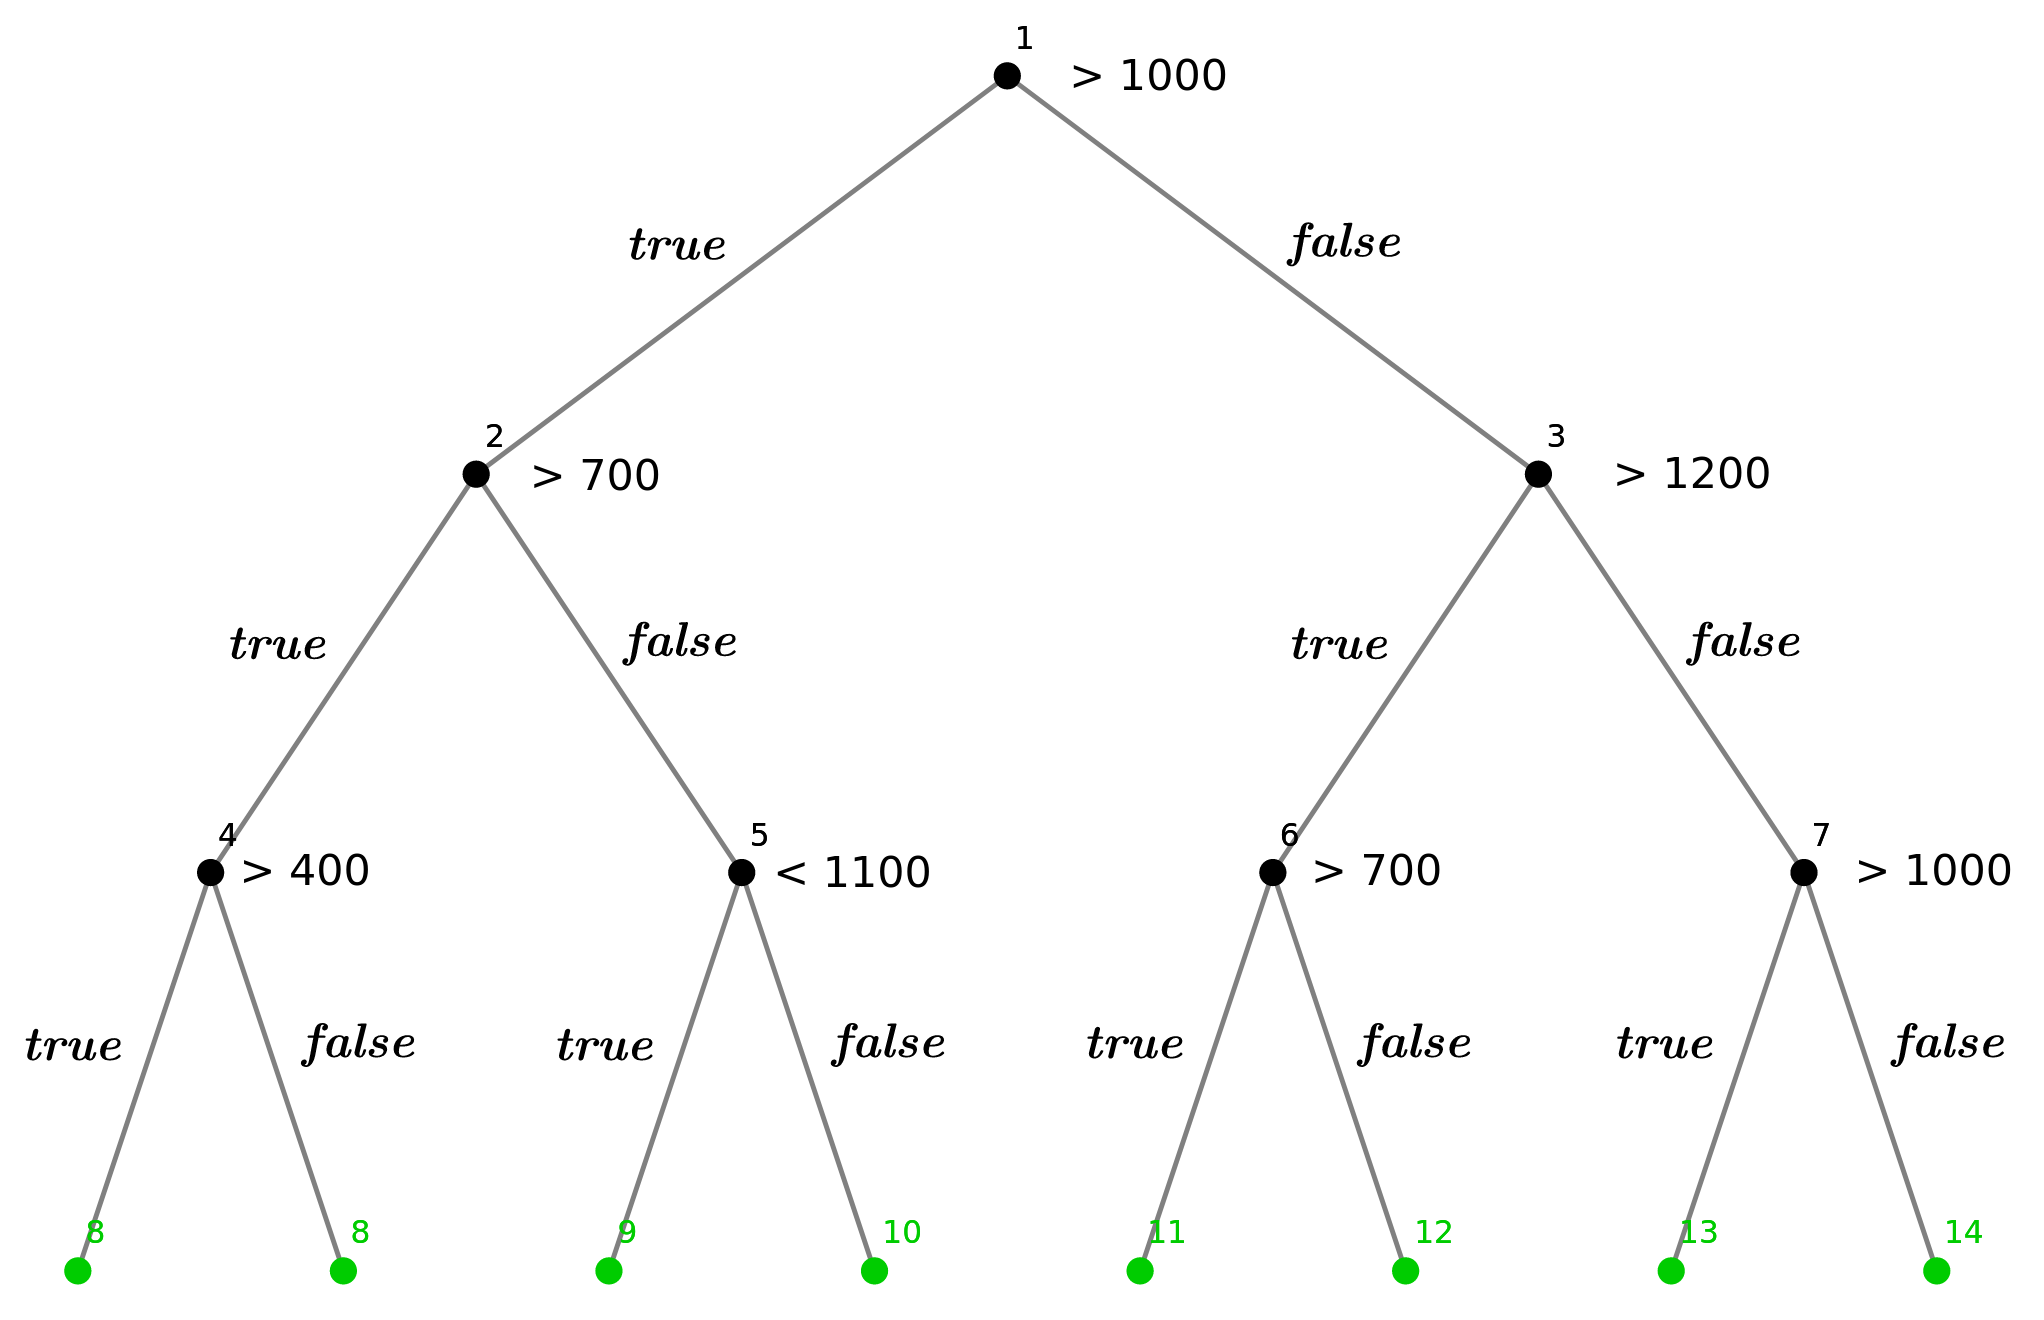
\includegraphics[width=\linewidth]{stablo_primer_1.png}
    \caption{Stablo stanja simboličkog izvršavanja koje odgovara primeru \ref{lst:primer_KLEE}. Zelenom bojom su označena završna stanja.}
    \label{fig:moj_primer}
\end{figure}

\begin{figure}
\noindent\begin{minipage}[t]{.45\textwidth}
\begin{lstlisting}
   void foo(int a) 
   {
     if (a > 1000) {
       a /= 2;
       if (a > 700) {
         a /= 2;
         if (a > 400) {
           a /= 2;
         }
         else {
           return ;
         }
       }
       else {
         a *= 2;
         if (a < 1100) {
           return ;
         }
         else {
           a *= 2;
         }
       }
     }
\end{lstlisting}
\end{minipage}\hfill
\begin{minipage}[t]{.45\textwidth}
\begin{lstlisting}
     else {
       a *= 2;
       if (a > 1200) {
         a /= 2;

         if (a > 700) {
           a /= 2;
         }
         else {
           return ;
         }
       }
       else {
         a *= 2;

         if (a > 1000) {
           a *= 2;
         }
         else {
           a *= 2;
         }
       }
     }
   }
\end{lstlisting}
\end{minipage}
\captionof{lstlisting}{Primer simboličkog izvršavanja u alatu KLEE}
\label{lst:primer_KLEE}
\end{figure}

\begin{figure}[ht]
    \centering
    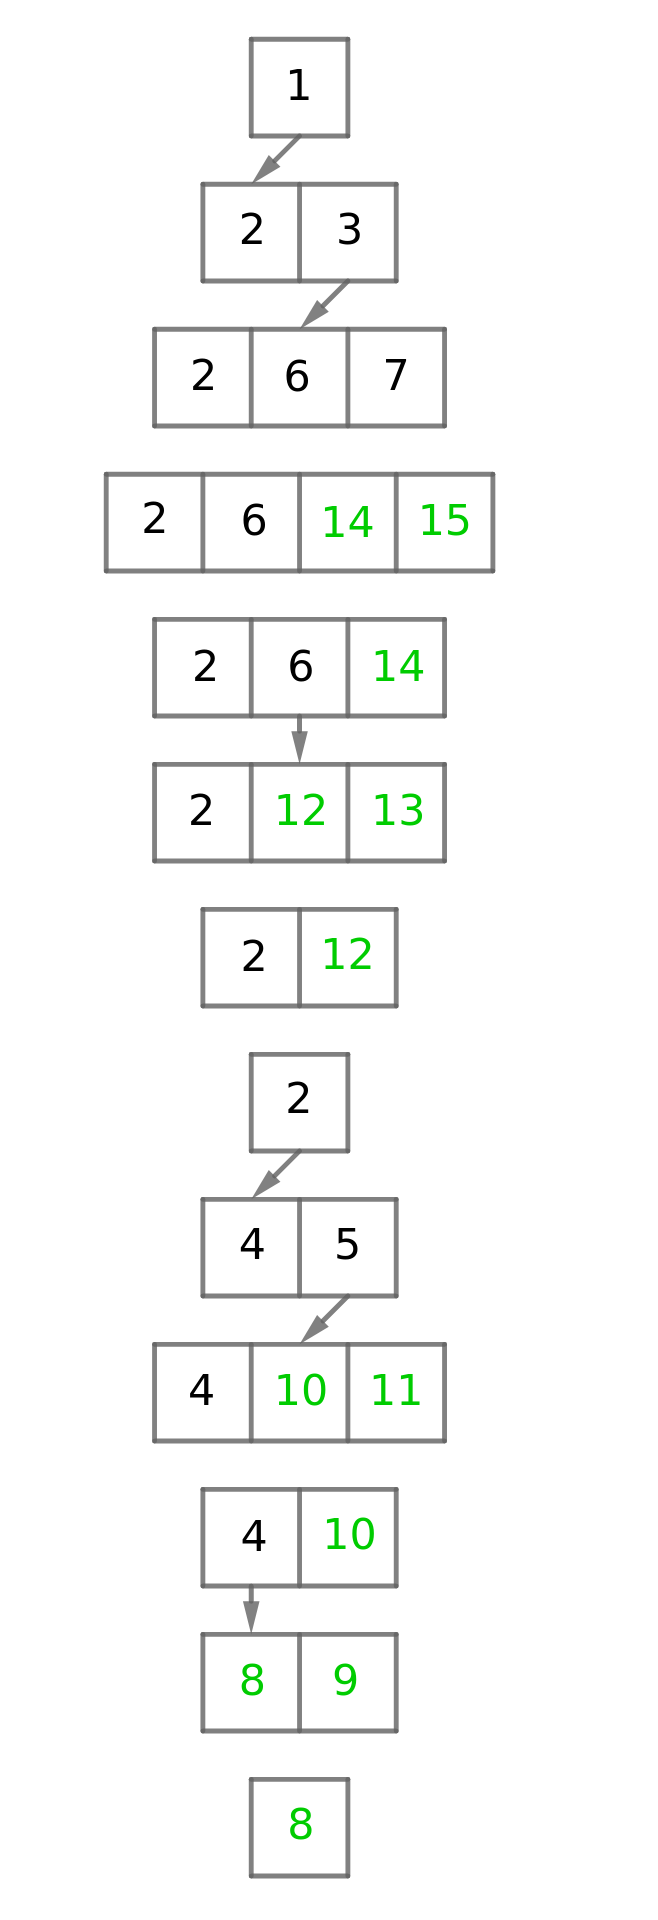
\includegraphics[height=1.09\linewidth]{DFS_states_1.png}
    \caption{Pregled izgleda reda stanja tokom izvršavanja DFS algoritma. Zelenom bojom su prikazana završna stanja, a strelice predstavljaju evoluciju stanja.}
    \label{fig:DFS_stanja}
\end{figure}

\subsection{DFS}
Na slici \ref{fig:DFS_stanja} je prikazano na koji način se menja niz stanja izvršavanjem algoritma pretrage stabla stanja u dubinu. Stanja odgovaraju primeru \ref{lst:primer_KLEE}.  Sa slike vidimo da se na početku kreće iz stanja 1 koje evoluira u stanje 2 i dodaje se novo stanje 3 na kraj niza. Međutim, onda se bira baš stanje 3, kao poslednje u nizu kako bi se simulirala pretraga grafa u dubinu. Nakon toga, stanje 3 evoluira u stanje 6 i dodaje se novo stanje 7, dok stanje 2 ostaje i dalje u nizu ali na početku. Pretraga se nastavlja iz stanja 7 koje evoluira u stanje 14 i dodaje se stanje 15. Kako je sledeće stanje koje se izvršava broj 15, a ono je ujedno i završno stanje, samo se izbacuje iz niza i prelazi se na stanje 14. Ono je takođe završno pa se pretraga vraća na stanje 6, čime se zapravo izvršio povratak na prethodno grananje (kod stanja 3 na slici). Iz stanja 6 se dobijaju 2 završna stanja, koja nakon izvršavanja bivaju izbačena iz niza gde ostaje samo stanje 2. Primećujemo da je cela desna polovina stabla stanja izvršena, tj. istražene su sve putanje, pa se pretraga dalje na isti način fokusira na levu plovinu stabla. Iako je u pitanju DFS algoritam koji jednu putanju izvršava do kraja pre nego što pređe na narednu, primećujemo da se sve vreme čuvaju i stanja koja su vezana za putanje koje se ne izučavaju u tom trenutku.

\begin{figure}[ht]
    \centering
    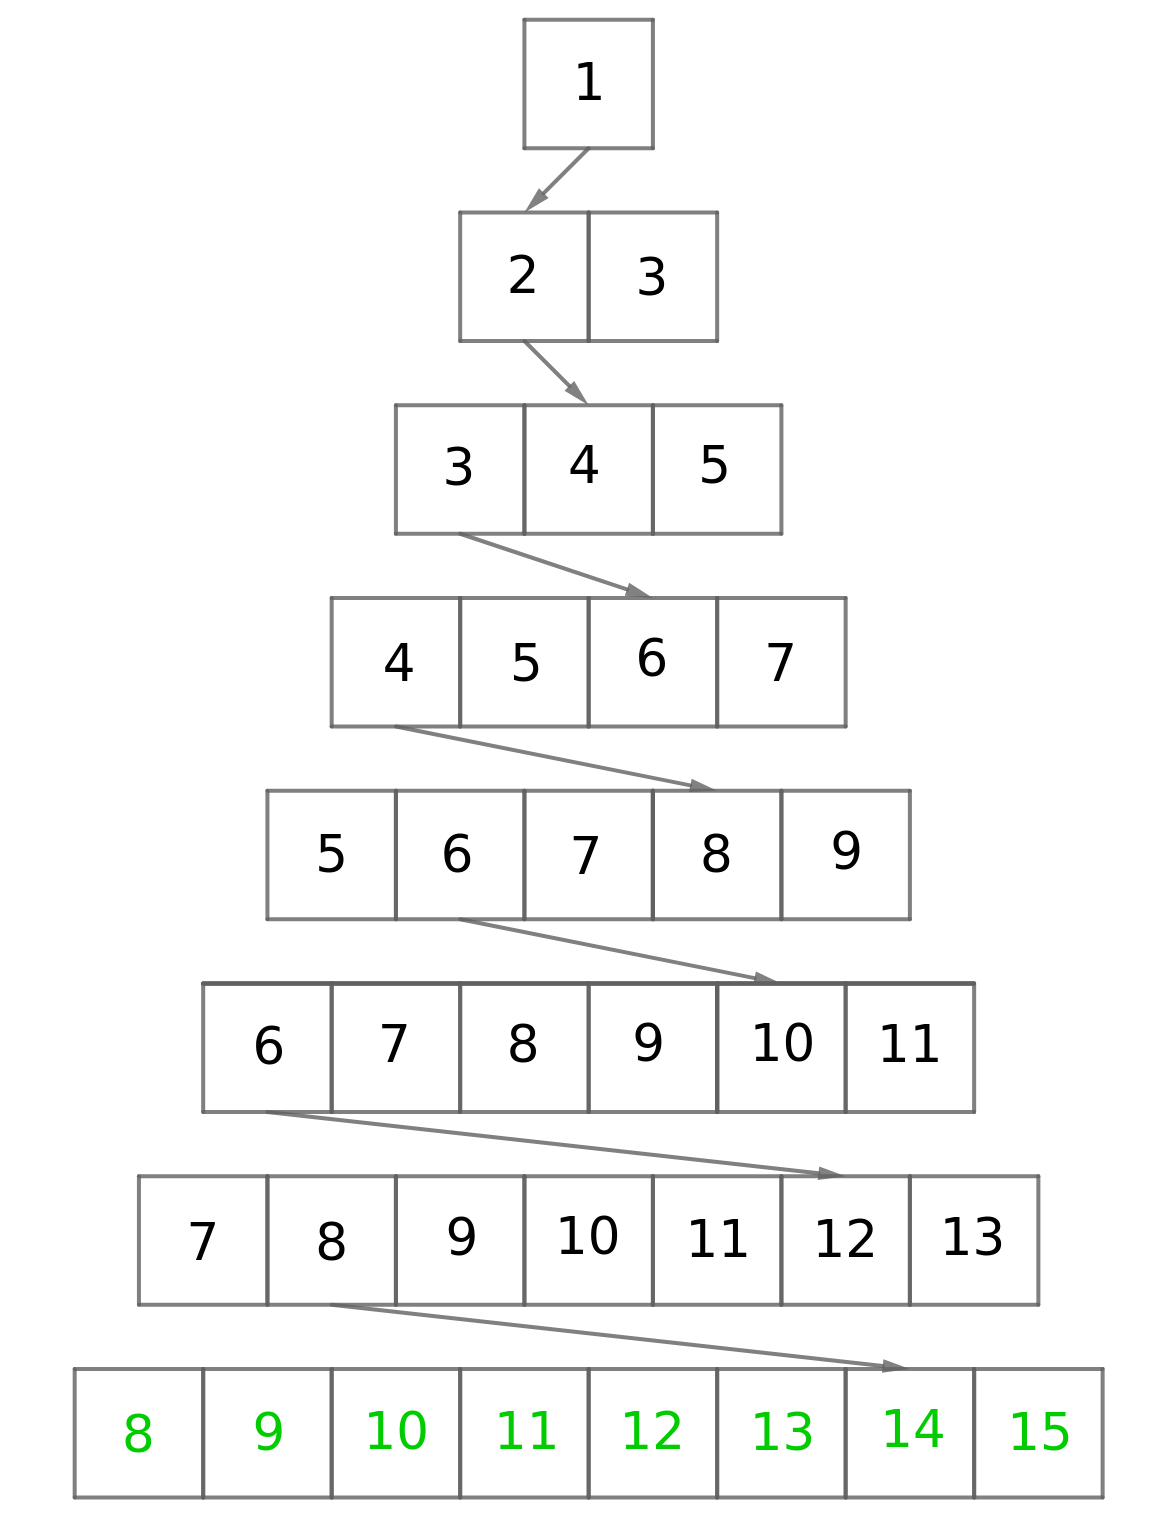
\includegraphics[width=0.6\linewidth]{BFS_stanja_1.png}
    \caption{Pregled izgleda niza stanja tokom izvršavanja BFS algoritma. Zelenom bojom su prikazana završna stanja, a strelice predstavljaju evoluciju stanja.}
    \label{fig:BFS_stanja}
\end{figure}
\bigbreak

\subsection{BFS} 
Zbog drugačije prirode algoritma i niz stanja se prilikom pretrage stabla stanja u širinu menja u drugačije u odnosnu na pretragu u dubinu. Ako pogledamo kako se na slici \ref{fig:BFS_stanja} menja red koji čuva stanja koja se izvršavaju vidimo da se kreće iz stanja 1. Zatim stanje 1 evoluira u stanje 2 i na kraj reda se dodaje stanje 3. Sledeće stanje koje se uzima je upravo 2, koje dalje evoluira u stanje 4. Takođe se dodaje novo stanje 5. Stanje 3 mora da ostane na početku reda kako bi bilo naredno izvršeno jer je u pitanju algoritam BFS i potrebno je prvo izvršiti sva stanja na jednom nivou stabla, pa tek onda preći na naredni. Od stanja 3 se dobijaju stanja 6 i 7 koji idu na kraj reda. Sledeće stanje koje se izvršava je 4, od koga nastaju 8 i 9. Postupak se nastavlja na prikazani način sve dok u redu ne ostanu samo završna stanja (8 - 15). U tom trenutku će se sva završna stanja izvršiti redom i biti izbacivana iz reda u redosledu izvršavanja. Pošto iz završnog stanja nema gde da se ode dalje, ono se samo izbacuje, time se putanja završava i prelazi se na naredno stanje  koje treba izvršiti.
% ------------------------------------------------------------------------------
\chapter{Ideja i implementacija algoritma BFS-DFS} \label{algoritam}
U ovom delu će biti opisan algoritam kojim je unapređen alat KLEE. Rezultati ovog algoritma će biti upoređeni sa rezultatima algoritma koji autori alata preporučuju kao \textit{najbolji}. Najbolji se u ovom kontekstu odnosi na algoritam koji postiže najveću moguću pokrivenost koda, uz razumno vreme izvršavanja. Poređenje rada ova dva algoritma je vršeno na korpusu programa koji je korišćen u okviru evaluacije samog rada \cite{klee}. U pitanju su netrivijalni programi, što pokazuje kako se alat ponaša prilikom provere ispravnosti realnog softvera. Implementacija algoritma BFS-DFS kao i korpusi korišćeni u evaluaciji se mogu naći na adresi \url{https://github.com/filozof50/master_rad}.

\section{Ideja algoritma} \label{ideja_algoritma}
Algoritam kojim je unapređen alat KLEE predstavlja kombinaciju dva grafovska algoritma. U pitanju su pretraga garafa u širinu (BFS) i pretraga grafa u dubinu (DFS). Kako u simboličkom izvršavanju postoji stablo stanja, ideja je upotrebiti neki algoritam pretrage grafa kako bi se izvršilo što više stanja. Ideja je iskoristiti dobre strane ova dva algoritma, a u najvećoj mogućoj meri anulirati njihove mane. 

BFS algoritam u ranoj fazi izvršavanj može otkriti neke anomalije u programu jer ide u širinu, međutim iz toga razloga i brzo puni memoriju. S druge strane DFS algoritmom je zauzeće memorije znatno manje, međutim problem predstavlja što se svaka putanja izučava do kraja. 

Ideja BFS-DFS algoritma je da se prvo krene pretragom u širinu, čime bi se stablo stanja u velikoj meri ,,razgranalo'' i bio bi začet veliki broj različitih putanja. Kako se memorija ne bi prepunila (usled čega dolazi do odbacivanja velikog broja stanja), u nekom trenutku se prelazi na DFS pretragu čime bi putanje trebalo da se izučavaju do kraja. Prelazak sa algoritma pretrage u širinu, na pretragu u dubinu se vrši nakon što je popunjena određeni procenat memorije koja je dodeljena alatu KLEE. Procenat memorije nakon kog se prelazi na pretragu u dubinu se određuje parametrom, prilikom pokretanja alata. 

U trenutku prelaska na DFS algoritam, stablo stanja je razgranato i započeto je izučavanje nekih putanja. Prelaskom na pretragu grafa u dubinu bi trebalo da se sve putanje izuče do kraja, jedna po jedna. Dakle, odabere se jedno stanje, i iz njega se pokreće pretraga u dubinu koja izučava putanju do samog kraja. Stanje iz kog se pokreće pretraga u dubinu je ono koje je najbliže nekoj naredbi koja do tada nije bila izvršena. Opravdanje za ovakav pristup leži u činjenici da je i vreme ograničeno, tj. da se prilikom pokretanja KLEE-a zadaje vreme u kome izvršavanje mora biti završeno. U suprotnom se izvršavanje prekida usled prekoračenja vremena. Ukoliko se uvek pri pokretanju pretrage u dubinu iz nekog stanja, tj. za neku putanju, bira stanje na opisani način, veće su šanse da će biti otkrivena neka nova naredba i samim tim će se povećati pokrivenost koda. 

S\^am algoritam pretrage grafa u dubinu ima problem u simboličkom izvršavanju sa petljama i rekurzijom gde broj iteracija odnosno rekurzivnih poziva zavisi od simboličke promenljive. Iz tog razloga se u predloženom algoritmu ne izučavaju putanje do samog kraja, već postoji odbacivanje nekih stanja. Odbacivanje stanja u svakom od algoritama koji su implementirani u alatu KLEE je neminovnost. Postoji ogorman broj stanja, ograničena memorija i vreme izvršavanja pa neka stanja moraju biti žrtvovana kada se radi o realnom softveru. U predloženom algoritmu se stanja odbacuju u sledećem slučaju: \\
Ako se izvršava pretraga grafa u dubinu za neku putanju, neka stanja se odbacuju kada se izvrši određen broj naredbi bez otkrivanja nove naredbe (naredba koja ranije nije bila već izvršena). Stanja koja se odbacuju su ona u kojima nije bila otkrivena nova naredba.


Ovo se radi po ugledu na odbacivanje stanja koje predlažu autori alata, koji takođe odbacuju stanja u kojima nije otkrivena nova naredba. Broj naredbi nakon kojih se vrši odbacivanje stanja se reguliše parametrom prilikom pokretanja alata KLEE. Nakon što jedna putanja bude izvršena do kraja, ili sva stanja iz nje budu odbačena, bira se novo stanje, odnosno nova putanja za koju se ponovo pokreće pretraga grafa u dubinu. Pseudo k\^od funkcije koja ilustruje opisan proces je zadat listingom \ref{lst:azuriraj_DFS}.

    \begin{lstlisting}[caption={Pseudo k\^od funkcije za ažuriranje DFS stanja},captionpos=b,label={lst:azuriraj_DFS}]
    function azuriraj_DFS_stanja(skup_novih_stanja, 
                                 skup_stanja_koja_treba_izbaciti):
      DFS_stanja.dodaj_na_kraj(skup_novih_stanja)
      DFS_stanja.ukloni(skup_stanja_koja_treba_izbaciti)        
            
      if broj_izvrsenih_stanja_bez_otrkivanja_nove_naredbe > 
         unapred_zadata_granica:
           for stanje u DFS_stanja:
             if !stanje.otkrivena_nova_naredba:
                DFS_stanja.ukloni(stanje)
    \end{lstlisting}

Ono što se dodatno radi u KLEE-u je da ako se memorija koja mu je dodeljena u potpunosti popuni, vrši se izbacivanje nekih stanja. Stanja koja se izbacuju se biraju slučajnom metodom, pri čemu se vodi računa da se ne izbacuju stanja u kojima je bila otkrivena nova naredba. Zanimljivo je da se samo jednom proverava da li je u nekom stanju otkrivena nova instrukcija. Ukoliko bi trebalo da bude izbačeno neko od aktivnih stanja i ustanovi se da je u njemu otkrivena nova instrukcija, slučajnom metodom se bira novo stanje i ono biva izbačeno, bez provere da li je u njemu bilo otkrivanja nove instrukcije. 

U algoritmu BFS-DFS do ovakvog izbacivanja stanja retko dolazi. Razlog je taj što se nakon  što se popuni određeni procenat memorije BFS-om, prelazi na DFS. A pretraga u dubinu je algoritam koji jako malo memorije puni stanjima. Eksperimentalno je pokazano da ukoliko je zadati procenat manji od 80\%, nikada neće doći do izbacivanja stanja na ovaj način. 

Nakon izvršavanja svakog stanja, ažuriranja skupa aktivnih stanja, se vrši provera da li je potrebno promeniti algoritam. Algoritam se menja samo ako se izvršava pretraga u širinu i ako je procenat memorije koja je popunjena veći od $P\%$ ukupne memorije koja je dodeljena alatu KLEE za rad. Vrednost $P$ je vrednost koju korisnik zadaje prilikom pokretanja alata i uzima vrednosti iz intervala $[0, 1]$. Pseudo k\^od funkcije koja vrši proveru popunjenosti memorije koja je dodeljena KLEE-u za rad je prikazan u lisitngu \ref{lst:popunjena_memorija}. Poslednje dve linije ovog koda su specifične za algoritam BFS-DFS i dodate su u implementaciji, dok je ostatak koda izvorni k\^od alata KLEE.

\begin{lstlisting}[caption={Pseudo k\^od funkcije koja proverava koliko je memorije popunjeno},captionpos=b,label={lst:popunjena_memorija}]
    function regulisi_iskoriscenost_memorije(aktivna_stanja, 
                                             nova_stanja,
                                    stanja_koja_treba_izbaciti):
      if popunjena_memorija >= memorija_dodeljena_alatu:
        X = slucajan_broj(0, aktivna_stanja.velicina())

        while X > 0:
          Y = slucajan_broj(0, aktivna_stanja.velicina())
          stanje = aktivna_stanja[Y]
          
          if stanje.otkrivena_nova_naredba:
            Y = slucajan_broj(0, aktivna_stanja.velicina())
            stanje = aktivna_stanja[Y]

          aktivna_stanja.ukloni(stanje)
          stanja_koja_treba_izbaciti.dodaj(stanje)
          
          if stanje in nova_stanja:
            nova_stanja.ukloni(stanje)
          X--
          
      if izvrsava_se_BFS i popunjena_memorija > zadate_granice:
        promeni_algoritam_na_DFS()
    \end{lstlisting}

U listingu \ref{lst:glavna} je prikazan pseudo k\^od glavne funkcije predloženog algoritma. Iz koda se vidi da se algoritam izvršava sve dok postoji barem jedno stanje koje može biti izvršeno ili dok ne dođe do prekida iz nekog drugog razloga. Do prekida može na primer doći usled prekoračenja vremena koje je određeno za simboličko izvršavanje određenog koda. 

Prvi korak je odabrati naredno stanje koje se izvršava. Naredno stanje se bira u zavisnosti od algoritma koji se izvršava u tom trenutku. Postoje dve kolekcije podataka u kojima se čuvaju stanja. Red stanja za BFS, i niz stanja za DFS. Ukoliko se izvršava algoritam BFS, za naredno stanje se uzima stanje sa početka reda stanja. S druge strane, ako je algoritam koji se u datom trenutku izvršava DFS, uzima se poslednje stanje iz niza stanja. 

  \begin{lstlisting}[caption={Pseudo k\^od glavne funckije algoritma},captionpos=b,label={lst:glavna}]
    function pokreni_pretragu(pocetno_stanje):
      aktivna_stanja.dodaj(pocetno_stanje)
            
      while aktivna_stanja.velicina() > 0:
        stanje = odaberi_stanje()
        nova_stanja, 
          stanja_koja_treba_izbaciti = izvrsi_stanje(stanje)
                
        regulisi_iskoriscenost_memorije(aktivna_stanja, 
                                        nova_stanja,
                               stanja_koja_treba_izbaciti)
        azuriraj_stanja(nova_stanja, stanja_koja_treba_izbaciti)
            
    \end{lstlisting}

U nekim situacijama se može desiti da je niz DFS stanja prazan. To je slučaj kad se tek prelazi na algoritam pretrage u dubinu, kada se neka putanja u potpunosti izuči do kraja, ili kada se sva stanja iz neke putanje izbace usled neotkrivanja nove naredbe. U toj situaciji je potrebno u niz stanja ubaciti početno stanje, tj. ono od kog se kreće istraživanje putanje u dubinu. Stanje koje se uzima je ono koje je najbliže nekoj do tada neposećenoj naredbi, što je prikazano u funkciji čiji je k\^od dat listingom \ref{lst:odaberi_stanje}.

\begin{lstlisting}[caption={Pseudo k\^od funkcije za odabir narednog stanja koje se izvršava},captionpos=b,label={lst:odaberi_stanje}]
    function odaberi_stanje():
      if izvrsava_se_BFS:
        return BFS_stanja[0]
      else:
        if DFS_stanja.velicina() > 0:
          return DFS_stanja[DFS_stanja.velicina() - 1]
        else:
            stanje = najblize_neposecenoj_naredbi(BFS_stanja)
            DFS_stanja.dodaj_na_kraj(trazeno_stanje)
            return trazeno_stanje
    \end{lstlisting}
    
Nakon što se odabere stanje koje će biti naredno izvršeno, ono se izvršava. Pseudo k\^od funkcije za izvršavanje stanja je prikazan u listingu \ref{lst:izvrsi_stanje}. Zavisno od naredbe koja se nalazi u stanju može doći do evolucije stanja ukoliko nije bilo grananja ili može doći do evolucije stanja uz kreiranje novog stanja ukoliko je došlo do grananja. Ukoliko nema grananja već samo evolucije stanja ono se smatra novim stanjem, odnosno dodaje se opet u skup aktivnih stanja tako evoluirano. Ovo se radi kako bi algoritmi koji su opisani u delu \ref{algoritmi} radili ispravno. Takođe, ukoliko je stanje bilo završno, može doći i do njegovog izbacivanja iz niza ili reda stanja jer završno stanje označava kraj putanje. Nakon što se neko stanje izvrši, vrši se ažuriranje skupa aktivnih stanja dodavanjem novonastalih ili brisanjem onih stanja koja su višak.

    \begin{lstlisting}[caption={Pseudo k\^od funkcije koja izvrsava stanje},captionpos=b,label={lst:izvrsi_stanje}]
    function izvrsi_stanje(stanje):
      izvrsi(stanje.trenutna_naredba)
      
      nova_stanja, stanja_koja_treba_izbaciti
      
      if stanje.jeste_grananje():
        evoulirano_stanje, novo_stanje = izvrsi_grananje(stanje)
        nova_stanja.dodaj(evoulirano_stanje)
        nova_stanja.dodaj(novo_stanje)
      
      if stanje.zavrsno:
        stanja_koja_treba_izbaciti.dodaj(stanje)
        
      return {nova_stanja, stanja_koja_treba_izbaciti}
    \end{lstlisting}
    
Kada se ustanovi koja su nova stanja dodata i koja bi trebalo da budu izbačena potrebno je ažurirati red, odnosno niz stanja, zavisno od algoritma koji se u trenutku izvršava. Nevezano od algoritma, sva nova stanja se dodaju na kraj i sva stanja koja je potrebno izbaciti se izbacuju iz odgovarajuće kolekcije (reda, odnosno niza). 

Ukoliko je algoritam koji se u trenutku izvršava pretraga grafa u dubinu dodatno se vrši i provera koliko je izvršeno naredbi od poslednje novootkrivene naredbe. Svaki put kada se počne DFS pretraga za neku putanju, ili kada se otkrije neka nova naredba, pamti se broj do data izvršenih naredbi. Prilikom svakog ažuriranja stanja u DFS nizu se proverava koliko je izvršeno naredbi do tog trenutka. Ukoliko je izvršeno $X$ naredbi od poslednje novootkrivene naredbe ili od trenutka pokretanja pretrage u dubinu za datu putanju, izbacuju se sva stanja u kojima nije bila otkrivena nova naredba. $X$ je vrednost koja se zadaje kao argumemt prilikom pokretanja alata KLEE, i mora biti pozitivan ceo broj. Pseudo kodovi funkcija za ažuriranje stanja su zadati listinzima \ref{lst:azuriraj_stanja}, \ref{lst:azuriraj_BFS} i \ref{lst:azuriraj_DFS}.

    \begin{lstlisting}[caption={Pseudo k\^od funkcije za ažuriranje stanja},captionpos=b,label={lst:azuriraj_stanja}]
    function azuriraj_stanja(skup_novih_stanja, 
                             skup_stanja_koja_treba_izbaciti):
      if izvrsava_se_BFS:
        azuriraj_BFS_stanja(skup_novih_stanja, 
                            skup_stanja_koja_treba_izbaciti)
      else:
        azuriraj_DFS_stanja(skup_novih_stanja, 
                            skup_stanja_koja_treba_izbaciti)
    \end{lstlisting}
    
    \begin{lstlisting}[caption={Pseudo k\^od funkcije za ažuriranje BFS stanja},captionpos=b,label={lst:azuriraj_BFS}]
    function azuriraj_BFS_stanja(skup_novih_stanja, 
                                 skup_stanja_koja_treba_izbaciti):
        BFS_stanja.dodaj_na_kraj(skup_novih_stanja)
        BFS_stanja.ukloni(skup_stanja_koja_treba_izbaciti)
    \end{lstlisting}
    
\section{Pregled najvažnijih klasa alata KLEE}
U ovom delu će biti opisano na koji način je implementiran alat KLEE, biće dat pregled najvažnijih klasa i metoda koje se koriste za simboličko izvršavanje u ovom alatu. Takođe će biti opisano na koji način je implementiran predloženi algoritam, koje su klase izmenjene, i na koji način.

K\^od u alatu Klee je organizovan u više direktorijuma koji pored osnovne implementacije sadrže i dokumentaciju, pomoćne skripte za bildovanje, razne vrste testova i primere. Fajlovi zaglavlja organizovani su u okviru foldera \texttt{klee/include} dok se osnova implementacije nalazi u okviru foldera \texttt{lib}. Specijalno \texttt{lib/Core} sadrži sve fajlove koji sadrže izvorne kodove za svaku od klasa koje su implementirane u okviru alata, i tu je smeštena implementacija BFS-DFS pretrage.

\subsection{Klasa \textit{Executor}}
Glavna i najvažnija klasa koja se koristi u KLEE-u je klasa \textit{Executor}. U ovoj klasi postoji metod \textit{run}. Jedini argument koji prima je inicijalno stanje, tj. početno stanje od koga se kreće u pretragu, koren stabla stanja. Unutar ove metode se pre svega kreira pretraživač (eng. \textit{Searcher}). 
Pretraživač je samo objekat klase koja zapravo vrši pretragu u stablu stanja. Jedna važna odlika ove klase je i vektor stanja koja se izvršavaju. U ovom vektoru se čuvaju sva aktivna stanja. Ukoliko tokom izvršavanja nekog stanja dođe do evolucije ili grananja, nova stanja se dodaju u skup aktivnih.

Glavni deo ovog metoda je petlja u kojoj se vrši kompletno izvršavanje (listing \ref{lst:glavna}). Ovaj metod uz priložen pseudo k\^od je prikazan u delu \ref{ideja_algoritma}.

Prilikom izvršavanja svake od naredbi se dodatno i menja logička formula koja se čuva u stanju. Logička formula u stanju odgovara uslovima koji važe za sve promenljive na nekoj putanji. Kada se dođe u neko stanje, putanja kroz k\^od je jedinstveno određena nizom stanja koja su prethodila tom stanju na putanji. Samim tim je i formula logike prvog reda jedinstveno određena za tu putanju, jer je ona nastala propagiranjem kroz niz stanja kojima se došlo u trenutno stanje. Ukoliko dolazi do evolucije stanja, formula se samo ažurira ukoliko ima potrebe za tim, a ako dođe do grananja, u stanju koje je evoluiralo dolazi do ažuriranja formule, dok se u novonastalom stanju nasleđuje formula iz stanja iz kog je ono nastalo kojoj se dodaje i uslova grananja. Za konjukciju i disjunkciju su implementirane klase u okviru alata.    
    
\subsection{Klasa \textit{ExecutionState}}
Klasa \textit{ExecutionState} predstavlja jedno stanje koje se izvršava. U ovoj klasi je najvažniji metod \textit{branch}, koji vrši grananje, tj. u kojem se prilikom grananja formira novo stanje. S druge strane, kako jedna instanca ove klase predstavlja stanje, u njoj postoji veći broj veoma zanimljivih atributa. Neki od njih su:

\begin{description}
    \item \textbf{\textit{pc}} - predstavlja narednu naredbu koja treba da bude izvršena.
    
    \item \textbf{\textit{prevPC}} - trenutna naredba koja se izvršava u stanju.
    
    \item \textbf{\textit{addressSpace}} - adresni prostor gde se smeštaju lokalne promenljive, pokazivači, nizovi koji su vezani za stanje.
    
    \item \textbf{\textit{constraints}} - ograničenja koja važe u stanju. Na osnovu njih se formira formula logike prvog reda, za koju se poziva SMT rešavač.
    
    \item \textbf{\textit{instsSinceCovNew}} - predstavlja broj naredbi koje su izvršene od poslednje novootkrivene naredbe.
    
    \item \textbf{\textit{coveredNew}} - govori o tome da li je u stanju otkrivena nova naredba. Ovaj atribut je veoma važan jer se na osnovu njega određuje koja stanja mogu biti izbačena iz skupa aktivnih kada dolazi do odbacivanja nekih stanja.
    
    \item \textbf{\textit{coveredLines}} - brojevi linija koje su pokrivene ovim stanjem i fajlovi u kojima se te linije nalaze. Na osnovu ovoga se može videti prilikom izvršavanja naredbe gde se ona nalazi u kodu.
    
    \item \textbf{\textit{symbolics}} - lista simboličkih promenljivih koje postoje u stanju. Zapravo predstavlja listu svih simboličkih promenljivih koje se nalaze na putu od korena stabla izvršavanja do čvora u kome se stanje nalazi.
\end{description}

\subsection{Klasa \textit{Searcher}} \label{pretrazivac}
Klasa \textit{Searcher} (pretraživač) je klasa koja služi kao glavna klasa za pretragu stabla stanja u alatu KLEE. Ovo je apstraktna klasa koja definiše važne metode koje mora da ima svaki od pretraživača. Izvedene klase su zapravo one koje koriste neki konkretan algoritam za pretragu stabla stanja. Tako razlikujemo \textit{DFSSearcher}, \textit{BFSSearcher}, \textit{RandomSearcher}, \textit{WeightedRandomSearcher} i \textit{RandomPathSearcher}, \textit{MergingSearcher}, \textit{BatchingSearcher} i \textit{InterleavedSearcher}. Takođe, dodata je potklasa \textit{BFSDFSSearcher} koja koristi algoritam koji je opisan u ovom radu. Važni metodi ove klase, samim tim i svih pretraživača odnosno izvedenih klasa su:
\begin{description}
    \item \textbf{\textit{selectState}} - čist virtuelni metod koji predefinišu sve potklase klase \textit{Searcher}, i koji služi za odabir narednog stanja koje će biti izvšeno.
    
    \item \textbf{\textit{update}} - čist virtuelni metod u kome se ažuriraju kolekcije podataka koje čuvaju stanja u pretraživaču, tj. vrši se dodavanje novih aktivnih stanja i uklanjaju se stanja koja više nisu aktivna. 
    
    \item \textbf{\textit{empty}} - čist virtuelni metod koji pruža informaciju o tome da li ima aktivnih stanja.
    
    \item \textbf{\textit{printName}} - virtuelni metod koji služi da se ispisše naziv pretraživača koji se koristi u pretrazi stabla stanja.
\end{description}

\section{Implementacija predloženog algoritma}
Kako bi mogao da bude implementiran novi algoritam u alatu KLEE, potrebno je i napraviti novu klasu. Ova klasa treba da nasleđuje apstraktnu klasu \textit{Searcher} i predefiniše njene važne metode koji su opisani u delu \ref{pretrazivac}. UML dijagram klase za klasu \textit{BFSDFSSearcher} je prikazan na slici \ref{fig:UML}.

\begin{figure}[ht]
    \centering
    \includegraphics[width=\linewidth]{dijagram_klase.png}
    \caption{Dijagram klase za novu implementiranu klasu BFSDFSSearcher.}
    \label{fig:UML}
\end{figure}

Atributi nove klase su dva vektora pokazivača na stanja. Jedan vektor služi za čuvanje stanja prilikom korišćenja algoritma pretrage grafa u dubinu, dok drugi služi kao dek, i njegova stanja se koriste kada je aktivan algoritam pretrage grafa u širinu. Dodatno postoji promenljiva koja govori o tome da li se izvršava BFS ili DFS algoritam. Postoji promenljiva koja definiše nakon koliko procenata popunjene memorije se prelazi na algoritam pretrage u dubinu. Takođe se čuva i referenca na objekat klase \textit{Executor}. Uloga ovog atributa će biti opisana u delu \ref{userSearcher}.

Pored metoda koje su nasleđene iz nastklase \textit{Searcher} u ovoj klasi postoji i nekoliko dodatnih metoda. Kako postoje dva algoritma koja se izvršavaju u ovom pretraživaču postoje posebne metode za ažuriranje odgovarjućih kolekcija stanja. Kada se pozove predefinisani metod za ažuriranje stanja, zavisno od algoritma koji se izvršava, poziva se odgovarajući metod za ažuriranje odgovarajuće kolekcije podataka. 

Takođe postoji metod koji pronalazi stanje u deku BFS stanja koje je najbliže nekoj neposećenoj naredbi. Ovaj metod se koristi prilikom prelaska sa algoritma pretrage grafa u širinu na algoritam pretrage u dubinu, odnosno kad se kreće u izučavanje neke putanje u dubinu. Kako bi se otkrilo koja putanja garantuje da će se najpre naći neka nova naredba koristi se ovaj metod. 

Još dva važna metoda su metod koji vrši promenu sa BFS-a na DFS, i metod koji vraća informaciju o tome da li se trenutno izvršava algoritam pretrage u dubinu. Ukoliko poslednje pomenuti metod vrati vrednost netačno (eng. \textit{false}), to znači da se trenutno izvršava pretraga u dubinu.

\section{Unapređenje postojećih klasa alata KLEE} \label{izmene}
Prilikom dodavanja novog algoritma za pretragu stabla stanja je bilo neophodno izmeniti neke klase u okviru implementacije alata KLEE. U ovom delu će za svaku klasu koja je promenjena biti opisane promene.

\begin{description}
    \item \textbf{\textit{Executor}} - u klasi \textit{Executor} je bilo neophodno dodati novi metod za brisanje aktivnih stanja. Metod koji postoji izbacuje neka stanja iz skupa aktivnih ukoliko dođe do prevelikog zauzeća memorije. Međutim, kako predloženi algoritam izbacuje stanja prilikom rada DFS algoritma, neophodno je izbaciti i ta stanja iz skupa aktivnih. Takođe, iz ove klase se pozivao metod za prelazak sa algoritma pretrage u širinu na algoritam pretrage u dubinu. U klasi \textit{Executor} je implementiran metod koji proverava koliko je memorije zauzeto. U ovom metodu je dodata i provera da li je procenat zauzete memorije veći ili jednak procentu memorije nakon čijeg punjenja se menja algoritam.
    
    \item \textbf{\textit{Searcher}} - u ovoj klasi je u enumeracionom tipu podataka dodat predloženi pretraživač. Enumeracioni tip čuva informaciju o tome koji su mogući pretraživači, a kako je dodat nov, bilo je neophodno dodati i njega u ovu listu.
    
    \item \textbf{\textit{UserSearcher}} \label{userSearcher} - u klasi \textit{UserSearcher} se vrši instanciranje novog pretraživača. Ova klasa je izmenjna tako što metod koji instancira pretraživač pored tipa pretraživača dobija i referencu na instancu klase \textit{Executor}. Ovo je urađeno jer je predloženom algoritmu neophodna ova referenca, zbog toga što algoritam poziva metod za izbacivanje nekih DFS stanja iz skupa aktivnih. Ovo je moglo biti urađeno tako što bi metod za izbacivanje stanja bio statički. Međutim, kako skup stanja nije statički atribut, odabrano je opisano rešenje. 
    
    U ovoj klasi je moguće definisati i dodatne parametre koji se prosleđuju alatu. Parametri kao što su algoritam koji se koristi u pretrazi, maksimalno dozvoljeno vreme izvršavanja, memorija koja je dodeljena KLEE-u i slično. Za potrebe predloženog algoritma, klasa je obogaćena sa dva parametra. Jedan čuva procenat memorije koji nakon što se popuni prelazi se na DFS (broj u pokretnom zarezu dvostruke tačnosti). Drugi je broj naredbi nakon kojih se izbacuju stanja iz DFS niza stanja ukoliko nije bilo otkrivanja nove naredbe (celobrojna vrednost).
\end{description}

Nijedna od navedenih izmena ne menja ponašanje alata KLEE. On se i dalje može koristiti na potpuno isti način kao i pre nego što je implementacija izmenjena dodavanjem novog algoritma.

\section{Upotreba algoritma BFS-DFS}

Kako bi predloženi algoritam mogao da se koristi u okviru alata KLEE, prilikom njegovog pokretanja je potrebno specifikovati da se radi o BFS-DFS pretrazi stabla stanja. Takođe je neophodno dodati i parametre koji određuju nakon koliko procenata popunjenosti dodeljene memorije dolazi do promene algoritma i broj izvršenih naredbi od poslednje otkrivene naredbe nakon kog dolazi do odbacivanja nekih stanja u algoritmu pretrage u dubinu. Parametar kojim se određuje procenat zauzeća memorije se zove \texttt{memory-part}, dok se parametar koji govori o broju naredbi nakon kojih se stanja izbacuju zove \texttt{insts-since-covered-new}. 

Primer pokretanja alata KLEE sa dodatnim parametrima je prikazano u listingu \ref{lst:pokretanje_klee_moj}.

\begin{lstlisting}[caption={Primer pokretanja alata KLEE gde se za pretragu stabla stanja koristi algoritam BFS-DFS.}, label={lst:pokretanje_klee_moj}, captionpos=b]
klee --write-cvcs --write-cov --max-memory=1000 external-calls=all
--only-output-states-covering-new --max-sym-array-size=4096 
--max-time=720min --search=bfs-dfs memory-part=0.4 
insts-since-covered-new=10000 mkdir.bc --sym-args 0 1 10 --sym-args 
0 2 2 --sym-files 1 8 --sym-stdin 8 --sym-stdout

\end{lstlisting}

Izlaz koji kreira alat, koji je već opisan u \ref{instalacija}, je potpuno isti kao i pre dodavanja novog algoritma. Primer izlaza alata za program \textit{mkdir} je prikazan na slici \ref{fig:my_mkdir}.

\begin{figure}[ht]
    \centering
    \includegraphics[width=\linewidth]{my_mkdir.png}
    \caption{Izlaz alata KLEE za izvršavanje programa \textit{mkdir} GNU Coreutils-a korišćenjem algoritma BFS-DFS.}
    \label{fig:my_mkdir}
\end{figure}

\section{Eksperimentalna evaluacija}
Poređenje predloženog algoritma i algoritma koji preporučuju autori alata je vršeno na odabranom korpusu programa iz GNU Coreutils-a. Predlog autora KLEE-a \cite{klee} je algoritam slučajne pretrage koji koristi heuristiku otkrivanja najbliže neposećene naredbe. 

\subsection{GNU Coreutils}
GNU Coreutils predstavlja skup alata za rad sa fajlovima, manipulaciju tekstom, komande komandne linije. Svi alati i komande su implementirane u programskom jeziku C \cite{coreutils}. Neke od komandi koje su implementirane su 

\begin{enumerate}
    \item \textit{ls} - komanda koja služi za izlistavanje sadržaja direktorijuma
    
    \item \textit{mv} - komanda koja se koristi za premeštanje fajlova iz jednog direktorijuma u drugi
    
    \item \textit{cp} - komanda koja omogućava kopiranje fajlova iz jednog direktorijuma u drugi
    
    \item \textit{printf} - komanda koja omogućava formatiran ispis
    
    \item \textit{kill} - komanda koja služi za slanje signala procesima kako bi bili prekinuti
    
    \item \textit{pwd} - komanda kojom se ispisuje apsolutna putanja do trenutnog direktorijuma
\end{enumerate} 

\subsection{Izbor parametara}
Na osnovu predloga autora \cite{klee}, alatu je dato 1000 megabajta memorije za izvršavanje. Maksimalno vreme izvršavanja je 12 sati. Svi eksperimenti su izvršavani na računaru sa procesorom Intel(R) Core(TM) i7-8550U od 1.80GHz, sa 8GB RAM memorije i sa operativnim sistemom LinuxMint 19.

Eksperimantalnim putem je pokazano da su najbolji parametri za pokretanje algoritma BFS-DFS 40\% za memoriju nakon čije popunjenosti se prelazi na pretragu u dubinu i 10000 za broj naredbi nakon kojih se vrši izbacivanje DFS stanja ukoliko nije bilo otkrivanja nove naredbe. Ukoliko se procenat zauzeća memorije poveća na preko 80\% dolazi do izbacivanja stanja usled potpunog zauzeća memorije. Eksperimetni su vršeni sa 85\%, 80\%, 67\%, 60\%, 40\% i 20\%. Menjanjem vrednosti ovog parametra se pokazalo da pokrivenost koda opada. Vrednosti koje su testirane za broj naredbi su 5000, 7000, 10000 i 15000. Vrednosti manje od 10000 su dovodile od manje pokrivenosti koda, dok je veća vrednost popravljala pokrivenost neznatno uz značajno veći utrošak vremena.

Eksperimentalno je pokazano da uz ovakav izbor parametara na odabranom korpusu programa nikada ne dolazi do popunjavanja memorije u potpunosti, odnosno da se stanja izbacuju iz skupa aktivnih samo DFS algoritmom na opisani način.

Pored opisanog pristupa, bilo je pokušaja neznatne modifikacije algoritma. Pokušaj je bio da se stanja ne izbacuju nakon određenog broja izvršenih naredbi pri čemu nije bilo otkrivanja nove, već da se izbacivanje vrši nakon određenog vremena, ukoliko nije bila otkrivena nova naredba. Još jedna ideja je bila da se nakon određene dubine u putanji ukoliko nije bilo otkrivanja nove naredbe vrši izbacivanje stanja. Nijedan od ova dva pristupa nije doneo unapređenja algoritmu.

\subsection{Rezultati evaluacije}

Na slikama \ref{fig:poredjenje_vemena_1} i \ref{fig:poredjenje_vemena_2} se vide rezultati poređenja vremena predloženih algoritama. Na osnovu rezultata se može videti da je u najvećem broju slučajeva algoritam BFS-DFS brži od slučajne pretrage sa heuristikom, negde i nekoliko puta. Takođe, u dva slučaja algoritam slučajne pretrage nije uspeo da se završi u predviđenom vremenu. Kod algoritma BFS-DFS se to nijednom nije desilo. 

Na slici \ref{fig:poredjenje_instrukcija} se mogu videti rezultati poređenja pokrivenosti naredbi (u procentima), dok slika \ref{fig:poredjenje_grana} prikazuje rezultate poređenja pokrivenosti grana (u procentima). Rezultati pokazuju da na odabranom korupusu programa slučajna pretraga sa heuristikom u proseku daje nešto veću pokrivenost koda, međutim ako se gleda na pojedinačnim programima, ovaj algoritam je u 50\% slučajeva davao veću pokrivenost naredbi.

\begin{figure}[H]
    \centering
    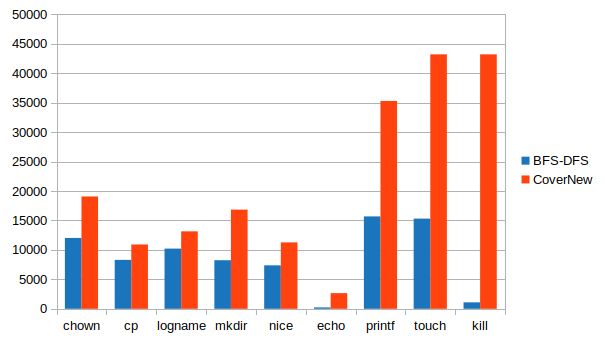
\includegraphics[width=1.0\linewidth]{poredjenje_vremena_1.png}
    \caption{Poređenje vremena (u sekundama) rada algoritama na korpusu programa iz GNU Coreutils-a. Kod programa kill i touch je došlo do prekoračenja vremena algoritmom slučajne pretrage sa heuristikom (12 sati) i usled toga je izvršavanje prekinuto.}
    \label{fig:poredjenje_vemena_1}
\end{figure}

\begin{figure}[H]
    \centering
    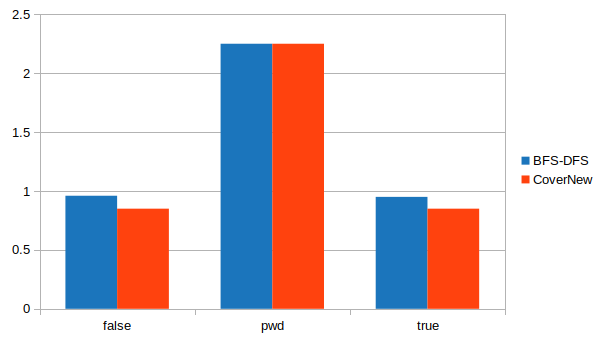
\includegraphics[width=1.0\linewidth]{poredjenje_vremena_2.png}
    \caption{Poređenje vremena (u sekundama) rada algoritama na korpusu programa iz GNU Coreutils-a.}
    \label{fig:poredjenje_vemena_2}
\end{figure}

\begin{figure}[H]
    \centering
    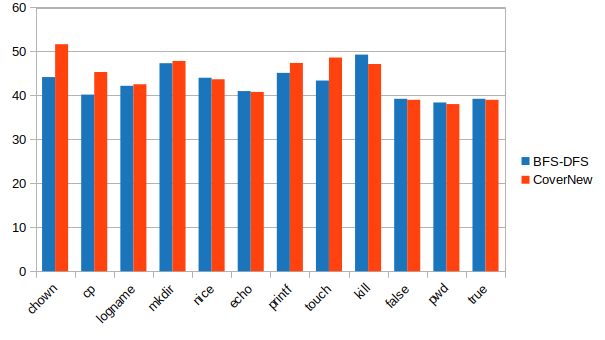
\includegraphics[width=1.0\linewidth]{poredjenje_instrukcije.png}
    \caption{Poređenje procenta pokrivenosti naredbi prilikom rada algoritama na korpusu programa iz GNU Coreutils-a.}
    \label{fig:poredjenje_instrukcija}
\end{figure}

\begin{figure}[H]
    \centering
    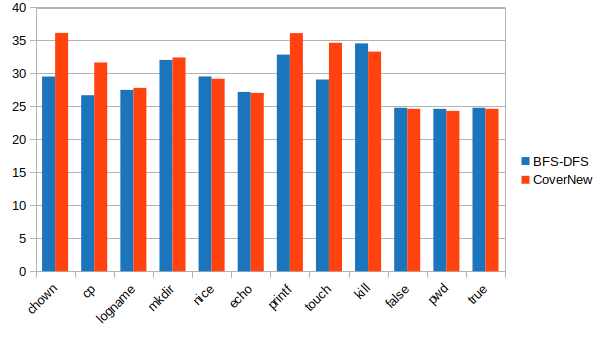
\includegraphics[width=1.0\linewidth]{poredjenje_grananja.png}
    \caption{Poređenje procenta pokrivenosti grana prilikom rada algoritama na korpusu programa iz GNU Coreutils-a.}
    \label{fig:poredjenje_grana}
\end{figure}

\newpage
Rezultati sprovedenog istraživanja i poređenja algoritma BFS-DFS sa algoritmom koji su predložili autori rada su pokazali da je opisanim pristupom, gde se kombinuju pretraga grafa u širinu (da bi se stablo što brže razgranalo) i pretraga grafa u dubinu (kako bi se putanje izučile što dublje je moguće), može uštedeti na vremenu pri čemu se ne gubi previše na pokrivenosti koda. U tabeli \ref{tab:tabela_rezultata} se mogu videti razlike vremena, kao i pokrivenosti naredbi i grana za algoritme BFS-DFS i slučajne pretrage sa heuristikom.

\begin{table}
{\rowcolors{3}{gray!80!white!40}{gray!80!white!65}
\begin{tabular}[caption={Osnovni primer simboličkog izvršavanja},captionpos=b,label={lst:tabela_rezultata}]{ |M{2cm}||M{2.5cm}|M{4.3cm}|M{4.3cm}| }
 \hline
 \multicolumn{4}{|c|}{Rezultati poređenja algoritama} \\
 \noalign{\global\arrayrulewidth=0.2mm}
 \hline
 Komanda& Razlika u vremenu (s)& Razlika u pokrivenosti naredbi (\%) & Razlika u pokrivenosti grana (\%)\\
 \hline
 chown& \textbf{-8037.34}& -7.48& -6.63 \\ \arrayrulecolor{black}\hline
 cp& \textbf{-2607.58}& -5.15& -4.97 \\\hline
 echo& \textbf{-2428.85}& \textbf{0.2}& \textbf{0.14} \\\hline
 false& 0.11& \textbf{0.22}& \textbf{0.16} \\\hline
 kill& \textbf{-42099.65}& \textbf{2.14}& \textbf{0.24} \\\hline
 logname& \textbf{-2933.87}& -0.35& -0.31 \\ \hline
 mkdir& \textbf{-8579.38}& -0.51& -0.38 \\ \hline
 nice& \textbf{-3888.14}& \textbf{0.36}& \textbf{0.34} \\ \hline
 printf& \textbf{-19599.61}& -2.26& -3.26 \\ \hline
 pwd& 0.12& \textbf{0.36}& \textbf{0.33} \\ \hline
 touch& \textbf{-27890.6}& -5.24& -5.57 \\ \hline
 true& 0.1& \textbf{0.22}& \textbf{0.16} \\
 \hline
\end{tabular}}
\caption{\label{tab:tabela_rezultata}Poređenje algoritama na korpusu programa iz GNU Coreutils-a. Tabela predstavlja poređenje algoritma BFS-DFS u odnosu na sučajnu pretragu sa heuristikom. Svaka vrednost je dobijena oduzimanjem vrednosti za slučajnu pretragu od njoj odgovarajuće vrednosti koja je dobijena algoritmom BFS-DFS. Podebljane vrednosti pokazuju gde je algoritam BFS-DFS bio bolji u odnosu na slučajnu pretragu sa heuristikom.}
\end{table}

% ------------------------------------------------------------------------------
\chapter{Zaključak}
% ------------------------------------------------------------------------------
U ovom radu su opisani opšte tehnike i načini verifikacije softvera sa posebnim osvrtom na statičku verifikaciju softvera, konkretno na simboličko izvršavanje. Simboličko izvršavanje je jedna od danas često 
primenjenih tehnika statičke verifikacije softevra, a koristi se i u najvećim softverskim kompanijama. Za rad je odabran alat KLEE, zasnovan na simboličkom izvršavanju, koji je obogaćen novim algoritmom pretrage stabla stanja.

Osnovna ideja rada je kombinovanje dva osnovna algoritma pretrage grafova kako bi se u kontekstu simboličkog izvršavanja iskoristile njihove dobre strane. Poznati problemi koje imaju ovi algoritmi pojedinačno nisu u potpunosti rešeni, ali su u velikoj meri uspešno prevaziđeni. Predloženi algoritam je na programima koji su napisani u okviru GNU Coreutils-a, poređen sa algoritmom koji su autori rada predložili kao najbolji u smislu pokrivenosti koda i sveukupnih performansi. Rezultati su pokazali da se ovim pristupom može značajno uštedeti na vremenu, pri čemu je pokrivenost koda nešto manja.

Dalja unapređenja bi podrazumevala nešto drugačiji pristup i modifikaciju algoritma. Kombinacija BFS i DFS algoritma bi mogla da se izmeni tako što se nakon nekog vremena, tj. ponovnog pražnjenja memorije završavanjem putanja pretragom u dubinu, ponovo prelazi na pretragu u širinu. Na ovaj način bi se stablo izvršavanja dodatno razgranalo na nekom nivou čime bi potencijalno nastale neke nove zanimljive putanje.
% ------------------------------------------------------------------------------
% Literatura
% ------------------------------------------------------------------------------
\printbibliography[heading=bibintoc,title=\foreignlanguage{serbian}{Literatura}]

% ==============================================================================
% Završni deo teze i prilozi
\backmatter
% ==============================================================================

% ------------------------------------------------------------------------------
% Biografija kandidata
\begin{biografija}
\textbf{Strahinja S. Stanojević} rođen je 16.05.1995. godine u Kosovskoj Mitrovici. Osnovnu školu, kao i prirodno-matematički smer gimnazije u Grockoj, završio je kao nosilac Vukove diplome. 

Smer Informatika na Matematičkom fakultetu Univerziteta u Beogradu upisuje 2014. godine. Na navedenom smeru je diplomirao 2017. godine, posle tri godine studija sa prosečnom ocenom 9,34. Master studije upisuje na istom fakultetu odmah nakon diplomiranja. 

U oktobru 2018. biva izabran u zvanje „Saradnik u nastavi“ na Matematičkom fakultetu paralelno sa master studijama. Drži vežbe iz kurseva „Konstrukcija i analiza algoritama” na smerovima ,,Računarstvo i informatika'' i ,,Informatika'', kao i ,,Programiranje 1'' na prvoj godini osnovnih studija smera ,,Informatika''. 

Oblasti interesovanja uključuju pre svega razvoj i verifikaciju softvera i algoritme.
\end{biografija}
% ------------------------------------------------------------------------------

\end{document} 